\chapter{Dynamical Systems Formulation of the Extraction Architecture}
\label{ch:lagrangian}

\begin{definition}[Epistemological Status of This Chapter]
This chapter formalizes the extraction architecture as an optimal control problem governed by Lagrangian mechanics. The framework establishes a substrate-independent dynamical homology: distinct systems exhibit equivalent governing equations once their state variables and constraints are operationalized. It does not assert that social quantities are measured in Volts or Teslas. distinct systems exhibit equivalent governing equations once their state variables and constraints are operationalized. Quantitative finance uses the heat diffusion equation to model stock options without measuring capital in degrees Kelvin; this framework uses the mathematics of optimal control theory, fractional calculus, and circuitry because both physical networks and socioeconomic architectures optimize energy, labor, and suppression under structural constraints. All claims are assigned confidence tiers consistent with the Empirical Methodology chapter (p.~\pageref{ch:empirical_methodology}).
\end{definition}

The hardware layer established in Chapter~\ref{ch:system_init} maps the extraction system onto a series RLC topology. The software layer formalizes the five-tier hierarchy, the Complex Wage, and the Interference Engine. This chapter supplies the unifying root equation that governs both layers. The augmented Lagrangian $\mathcal{L}^*$ compresses the kinetic capacity of the masses, the engineered constraint field of the Elite, the dissipative friction of the state, and the marginal cost of suppression into a single optimal control problem.

\section{The Augmented Lagrangian}

In Lagrangian mechanics, the state of a system is defined by its Kinetic Energy ($T$) and its Potential Energy ($V$). The action integral $S = \int \mathcal{L}\,dt$ is stationary along the path the system actually follows. The Elite configure the Potential ($V$), the masses supply the Kinetic labor ($T$), and the system executes the path of least action. The extraction architecture obeys the same optimization logic.

\subsection{The Isomorphism: $T$ and $V$}

\begin{itemize}
    \item \textbf{Kinetic Energy ($T$):} The Kinetic Capacity $K(t)$ of the Out-group and Buffer Class, representing class-solidarity energy, drift velocity, and the physical capacity for resistance.
    \item \textbf{Potential Energy ($V$):} The Lyapunov Energy Ceiling $V(q)$ and the Navigation Function $\varphi_i(q)$ act as the potential field. The Elite ($E$) engineer the legal, spatial, and psychological potential well that traps the population.
\end{itemize}

The Elite do not micromanage every individual. They engineer the potential field $V(q)$ and allow the system dynamics to execute the extraction.

\subsection{The Rayleigh Dissipation Function}

Standard Lagrangian mechanics models conservative systems, but the framework explicitly features friction: the Resistor $R$, bureaucratic friction, stop-and-frisk policing, and administrative drag. The Rayleigh Dissipation Function $\mathcal{D}$ incorporates this non-conservative dissipation into the Euler-Lagrange formalism:
\begin{equation}\label{eq:lag-euler-lagrange}
\frac{d}{dt}\left(\frac{\partial \mathcal{L}}{\partial \dot{q}_i}\right) - \frac{\partial \mathcal{L}}{\partial q_i} + \frac{\partial \mathcal{D}}{\partial \dot{q}_i} = Q_i
\end{equation}
where $\mathcal{D}$ represents the thermodynamic heat loss exacted by the state upon the Out-group, and $Q_i$ represents external coercive forces applied by the Enforcement Class ($F_{\text{enforce}}$).\footnote{This equation is classified as Tier~3 (ordinal/structural); the Euler-Lagrange formulation with Rayleigh dissipation is a published result of classical mechanics applied to the framework's operationalized state variables. See the Empirical Methodology chapter (p.~\pageref{ch:empirical_methodology}) and Appendix~\ref{app:empirical_index}.}

\subsection{The Augmented Form}

The canonical kernel objective is an optimization problem: $\max E(t)$ subject to the constraint $M_{\text{eff}}(t) < \tau$. In classical mechanics, systems subjected to constraints are solved using Lagrange Multipliers ($\lambda$). The augmented Lagrangian is:
\begin{equation}\label{eq:lag-augmented}
\boxed{\mathcal{L}^*(q, \dot{q}, t) = T(\dot{q}, t) - V(q, t) - \mathcal{D}(q, \dot{q}, t) + \lambda\bigl(\tau - M_{\text{eff}}(t)\bigr)}
\end{equation}
\footnote{This equation is classified as Tier~3 (ordinal/structural); the augmented Lagrangian formalizes the directional claim that the Elite optimize extraction subject to a rebellion-threshold constraint. See the Empirical Methodology chapter (p.~\pageref{ch:empirical_methodology}) and Appendix~\ref{app:empirical_index}.}

The terms map onto the framework as follows:
\begin{itemize}
    \item \textbf{$T$ (Mobilized Social Capacity):} The kinetic energy of the Out-group and Buffer class attempting to move upward or organize.
    \item \textbf{$V$ (Engineered Constraint Field):} The systemic diodes, redlining boundaries, and Lyapunov ceilings the Elite construct to trap that momentum.
    \item \textbf{$\mathcal{D}$ (Rayleigh Dissipation):} The social heat loss, exhaustion, administrative drag, and the friction of stop-and-frisk policing. This term formalizes the Resistor $R$ documented in Section~\ref{subsec:resistor}.
    \item \textbf{$\lambda$ (Marginal Cost of Suppression):} Setting the constraint $M_{\text{eff}}(t) < \tau$ means $\lambda$ equals the systemic cost $W = \psi_m + j\psi_s$. It calculates the capital and psychological wage the Elite must expend at any moment to enforce the boundary.
\end{itemize}

The Complex Wage $W = \psi_m + j\psi_s$ (Equation~\ref{eq:2.2b-complex-wage-def}) resolves the Lagrange multiplier into its real and imaginary components. The material wage $\psi_m$ is the real-power expenditure; the psychological wage $j\psi_s$ is the reactive-power expenditure that stores energy in the cultural field and deflects class momentum orthogonally.

\section{The Principle of Least Action and Autonomous Propagation}

In physics, the Principle of Least Action ($\delta S = 0$) dictates that a system evolves along the path that minimizes the action integral $S = \int \mathcal{L}\,dt$. Applied to the framework, this explains the Autonomous Propagation (Mode 2) of the extraction architecture. The Buffer Class ($I_{\text{buffer}}$) does not need to harbor conscious malice. The Buffer Class takes the path of least resistance through the socioeconomic potential well designed by the Elite. Because the Elite set the boundary conditions to make solidarity infinitely costly---the $\delta$-threshold of the psychological wage---the path that minimizes action naturally leads to the extraction outcome.

The Euler-Lagrange dynamics therefore describe the motion of the Out-group and the default trajectory of the Buffer Class. The path of least action through an engineered potential well is the formal statement of why the extraction algorithm propagates without requiring explicit coordination from $E$ at every node.

\section{Three Falsifiability Experiments}

The framework becomes falsifiable because it produces measurable parameters, observable time-series behavior, rival-model tests, and historical predictions. The following three experiments test the Lagrangian terms against the 500-year dataset.

\subsection{Experiment 1: Proving Rayleigh Dissipation ($\mathcal{D}$) via State Friction}

\textbf{The Claim:} Bureaucratic drag, redlining, and policing act as thermodynamic friction ($\mathcal{D} = I^2R$) that dissipates the kinetic momentum ($T$) of the Out-group into useless heat (exhaustion, legal fees, lost time).

\textbf{The Data Query:} Isolate two historical cohorts of the Out-group with identical initial starting capital (Potential $V$) and labor participation (Kinetic $T$). Measure a period where the state abruptly increased $\mathcal{D}$ (e.g., the introduction of Stop-and-Frisk in NYC, or the 1994 Crime Bill).

\textbf{The Test:} If the physics hold, the rate of economic upward mobility (the velocity $\dot{q}$) must drop in exact mathematical proportion to the increase in state friction (arrest rates, average hours spent in court, asset forfeiture).

\textbf{Falsification:} If policing and bureaucratic friction increase massively, but the Out-group's net wealth accumulation and organizational momentum remain statistically unaffected, then $\mathcal{D}$ is not a true physical friction, and the model breaks.

\subsection{Experiment 2: Stress-Testing the Lagrange Multiplier ($\lambda$)}

\textbf{The Claim:} $\lambda$ represents the marginal cost of suppression. When the Out-group's effective mass/momentum ($M_{\text{eff}}$) approaches the systemic rebellion threshold ($\tau$), the Elite must drastically spike their expenditure ($\lambda$) to enforce the boundary.

\textbf{The Data Query:} Search for periods of massive Out-group kinetic mobilization: the 1968 Civil Rights momentum following MLK's assassination, the 1992 LA Uprising, or the 2020 BLM protests.

\textbf{The Test:} As $M_{\text{eff}}$ approaches $\tau$, track immediate Elite capital deployment: emergency federal grants to local police (the 1033 program militarization pipeline), sudden increases in corporate PR/diversity spending (the psychological wage deployed to pacify), and immediate legislative concessions.

\textbf{Falsification:} If massive riots and structural threats occur ($M_{\text{eff}} > \tau$) and the Elite do not alter their spending or control metrics ($\lambda$ remains flat), then the system is not actively optimizing a constraint, and the Lagrangian framework is falsified.

\subsection{Experiment 3: The Recompile Signature (Mode Shifts)}

\textbf{The Claim:} The Recompile is the Interface Swap executed by the Elite when raw kinetic suppression fails. The system swaps variables to maintain the same net extraction.

\textbf{The Data Query:} Analyze the transition from Jim Crow (pure physical constraint, high $V$) to the War on Drugs / Mass Incarceration (bureaucratic/legal friction, high $\mathcal{D}$).

\textbf{The Test:} If the Elite lowered the overt legal barriers ($V$) after the Civil Rights Act of 1964, the framework dictates they must have immediately increased the dissipation term ($\mathcal{D}$) to keep the Lagrangian $\mathcal{L}^*$ balanced. Quantify this by examining the Gini coefficient of racial wealth from 1965 to 1990. The net wealth extraction rate should remain relatively constant, smoothly transferring from the mechanics of $V$ (segregation) to $\mathcal{D}$ (incarceration and predatory lending).

\textbf{Falsification:} If the Civil Rights Act removed $V$ and $\mathcal{D}$ did not proportionately increase, the racial wealth gap would have closed permanently. If the gap closed and stayed closed, the Extraction Algorithm does not exist as a permanent physical law.

\subsection{Empirical Results}

The three experiments were executed against published administrative and survey datasets. Computational notebooks, curated data, and reproducible scripts are archived at \texttt{Paper/scripts/eq01a\_rayleigh\_dissipation.py}, \texttt{eq01b\_lagrange\_multiplier.py}, and \texttt{eq01c\_recompile\_signature.py}.

\paragraph{Experiment 1: Rayleigh Dissipation ($\mathcal{D}$).}
The directional test asks whether increased state friction correlates with suppressed Out-group economic mobility. Black incarceration per 100,000 rose 216\% from 1965 to 1990 (BJS administrative data). Over the same period, the Black/White median wealth ratio never exceeded 0.16 (Federal Reserve SCF and peer-reviewed historical reconstructions), indicating that kinetic momentum toward wealth accumulation was suppressed despite formal barrier removal. State-level cannabis arrest disparities (ACLU 2020) cluster in the Midwest and Northeast, regions with documented below-median Black economic mobility. The correlation between incarceration and Black unemployment is weak and negative ($r \approx -0.28$); business-cycle confounding dominates the short-term labor-market flow. The structural finding is the persistent wealth gap in the presence of massively expanded carceral friction. The framework is not falsified. \textbf{Confidence tier: Tier 2--3.}

\paragraph{Experiment 2: Lagrange Multiplier ($\lambda$).}
An event-study of three major mobilization waves tests whether Elite suppression expenditure spikes when $M_{\mathrm{eff}}$ approaches $\tau$.
\begin{itemize}
    \item \textbf{1968 (MLK assassination / 100+ city riots):} Protest intensity spiked 129\%. The Elite response was the FBI COINTELPRO ``Black Nationalist'' program expansion, a documented covert suppression expenditure increase.
    \item \textbf{1992 (LA Uprising):} Protest intensity spiked 367\%. Federal law-enforcement grants doubled immediately; the 1994 Crime Bill expanded carceral capacity, producing a 17\% increase in Black incarceration within three years.
    \item \textbf{2020 (George Floyd / BLM):} Protest intensity spiked 800\%, the largest protest wave in United States history. Federal grants spiked 2.5$\times$ (\$400M to \$1B); 1033 program transfers increased; police killings of Black Americans remained elevated.
\end{itemize}
In every documented case, $M_{\mathrm{eff}} \to \tau$ produced an observable $\lambda$ spike through legislative expansion, federal militarization grants, covert programs, or ideological pacification. No counter-example exists in the 1965--2024 dataset. The framework is not falsified. \textbf{Confidence tier: Tier 2--3.}

\paragraph{Experiment 3: Recompile Signature (Mode Shift).}
The mechanism-transfer test examines whether the Civil Rights Act of 1964 produced a compensatory increase in $\mathcal{D}$ as $V$ declined. The Black-White residential dissimilarity index fell from 0.78 (1964) to 0.56 (2020), a 28\% decline. Black incarceration rose 210\% over the same period. The two mechanisms are strongly negatively correlated ($r = -0.895$), consistent with a transfer between mechanisms; it is inconsistent with independent trends. The racial wealth gap remained open at approximately 6:1 to 8:1 across the full arc; no period of $V$ removal produced gap closure. Figure~\ref{fig:eq01c_recompile_signature} plots the three time series. The framework is not falsified. \textbf{Confidence tier: Tier 2.}

\begin{figure}[htbp]
\centering

\includegraphics[width=\textwidth]{figures/eq01/eq01c_recompile_signature.png}
\caption{\textbf{Experiment 3: Recompile Signature (1964--2020).} Panel A: Potential energy barrier $V$ (Black-White residential dissimilarity index) declined post-Civil Rights Act. Panel B: Rayleigh dissipation $\mathcal{D}$ (Black incarceration rate) rose as the mechanism transferred. Panel C: Extraction persistence (Black/White median wealth ratio) never closed. Data sources: BJS Prisoners series; Cutler-Glaeser-Vigdor segregation estimates; Federal Reserve SCF and Darity \& Mullen (2020) historical reconstructions.}
\label{fig:eq01c_recompile_signature}
\end{figure}

\paragraph{Synthesis.}
All three experiments produce directional results consistent with the augmented Lagrangian. The framework survives falsification on every test for which data exist. The strongest result is Experiment 3: the $V \to \mathcal{D}$ mechanism transfer is documented by a near-unit negative correlation between segregation and incarceration, with extraction (wealth gap) persisting throughout. The weakest result is Experiment 1, where business-cycle confounding obscures the short-term correlation between incarceration and unemployment; the structural finding (persistent wealth gap under expanded friction) remains stable.

\section{The QED Bridge: Explicitly Analogical}

The framework extends to the quantum layer by modeling ideology as systemic photon exchange. This extension is explicitly analogical and topological, not a literal quantum field theory derivation. Modern QED and particle physics are built on the Lagrangian Density ($\mathcal{L}_{\text{QED}}$). By defining the Lagrangian of the extraction field, the framework can formally derive the Systemic Feynman Diagrams and transition probability amplitudes outlined in Chapter~\ref{ch:algorithmic_epoch} from the principle of stationary action.

The Systemic Photon is redefined as a discrete Information Packet in the attention economy. Its energy is $E_{\text{photon}} = hf$, where $f$ is the algorithmic refresh rate and transmission frequency. Social media algorithms function as photon accelerators: they maximize $f$ and volume $\Phi$ simultaneously, driving reactive power $P = hf \cdot \Phi$ to arbitrarily high levels at near-zero material cost.

Stimulated emission is mathematically grounded in contagion/cascade dynamics on scale-free networks: when a highly clustered Buffer Class node receives a high-frequency input, the probability of passing that signal to neighbors approaches 1, creating a coherent, phase-locked cascade. Reverberation chambers are sociological lasers. The Elite seed an initial photon; stimulated emission produces a coherent, high-intensity beam of ideological radiation.

The QED extension therefore functions as an isomorphic mapping. It illustrates how systemic forces are mediated between nodes without physical contact. The heavy mathematical lifting of the framework remains rooted in the classical Lagrangian $\mathcal{L}^*$ and optimal control theory.

\section{Limits and Scope}

The Lagrangian $\mathcal{L}^*$ is a unification of existing model components, not a discovery of new physical laws. Its value is structural: it proves that the disparate scales of the framework---circuit models, optimal control dynamics, and quantum interaction layers---obey a single derivable root equation. The framework advances from metaphor to falsifiable dynamical modeling by specifying a Lagrangian control system, estimating its dissipative parameters, and validating its predicted spectral and transient responses against institutional data.

The model becomes falsifiable because it produces measurable parameters, observable time-series behavior, rival-model tests, and historical predictions. Its claim is dynamical homology; electromagnetic ontology is outside its scope.

\chapter{Redefining Racism}
\label{ch:redefining}

This book proposes a mathematical framework for understanding systems of oppression---social arrangements that systematically disadvantage a racialized Out-group ($O_{\text{racialized}}$) while advantaging an In-group ($I$), though the true beneficiaries are a small Elite class ($E \subset I$) that architects the system. The framework reveals a five-tier operational hierarchy: the Elite ($E$) extracts value, the Puppet Class ($P_{\text{uppet}}$) writes the laws, the Enforcement Class ($F_{\text{enforce}}$) physically actuates the extraction, the Buffer Class ($I_{\text{buffer}}$) receives a suppression allocation---status wages by default, escalating to material concessions when kinetic threat demands it, but always sourced from $O_{\text{racialized}}$ extraction---and $O_{\text{racialized}}$ bears the compounding burden of policy after policy. Traditional analyses of oppression often focus on individual prejudice or specific policy outcomes. Such approaches fail to capture the \textit{structural} dimensions of oppression: the recurring patterns, the self-reinforcing mechanisms, and the remarkable consistency of design across different systems and scales.

The central thesis of this book is that systems of oppression share a common \textbf{architecture of control}---a formal structure that can be identified mathematically regardless of the specific groups involved or the historical context. This architecture consists of:
\begin{enumerate}
    \item \textbf{Asymmetric autonomy restriction}: Policies and norms that constrain the Out-group's freedom---including physical movement, economic agency, and \textbf{reproductive autonomy}---while preserving the In-group's.
    \item \textbf{Selective empathy}: Validation of In-group suffering while dismissing or pathologizing Out-group harm.
    \item \textbf{Ideological justification}: Narratives that naturalize the asymmetry through spurious claims.
    \item \textbf{Resistance to structural critique}: Mechanisms that deflect analysis from the system to individual behavior.
\end{enumerate}

\paragraph{A note on formalism.}
The equations and set-theoretic notation deployed throughout this book function as \textit{precision-forcing devices}. They make the structure of an argument explicit and internally checkable, as formal logic does in philosophy; they are not empirical measurement instruments, as differential equations in physics are when parameters are derived from calibrated empirical data. Where empirical calibration is possible, it is offered and clearly marked; otherwise the qualifier ``ordinal'' or ``illustrative'' marks the boundary. The reader should interpret equations as structured claims about relative ordering and logical entailment. They are not quantitative predictions requiring parameter estimation. This book operates in the genre of \textit{formal diagnostic modeling}---a well-established register in political economy and critical theory. It does not claim the epistemological status of physical science.
The equations are calibrated against 146 anchor cases across 146 historical events; each calibration is assigned a confidence tier and a falsification criterion documented in Appendix~\ref{app:empirical_index}.

The Tri-Modal Enclosure Model ($\mathcal{S}_{\text{enc}}$,
Section~\ref{sec:trimodal}) is developed in Chapter~\ref{ch:system_init}. In
this chapter, racism supplies the first empirical specialization: the general
Out-group $O$ becomes $O_{\text{racialized}}$, and each enclosure mode is loaded
with historically specific racial mechanisms.

\section{The In-Group/Out-Group Binary as a Coarse Projection}
\label{sec:binary-refinement}

The conventional In-group/Out-group model is under-resolved.
It correctly identifies the first partition imposed by an oppressive system, but
it mistakes a low-resolution projection for the full architecture. The analytic move in this book retains the binary and increases its resolution.
At the first level of resolution, the population universe $U$ is partitioned into
an In-group $I$ and an Out-group $O$:

\begin{equation}\label{eq:binary-partition}
U = I \,\dot\cup\, O,
\qquad
I \cap O = \varnothing .
\end{equation}

This projection is useful but incomplete. It tells us where the primary
boundary is drawn, but not who designs the boundary, who administers it, who
physically enforces it, who receives status compensation for defending it, or
how the excluded population is internally fractured. The next operation is a
partition refinement:

\begin{equation}\label{eq:refined-five-tier-partition}
\operatorname{Refine}(I)
=
E \,\dot\cup\, P_{\text{uppet}} \,\dot\cup\, F_{\text{enforce}}
\,\dot\cup\, I_{\text{buffer}},
\qquad
E, P_{\text{uppet}}, F_{\text{enforce}}, I_{\text{buffer}} \subset I .
\end{equation}

The In-group is stratified: it contains the
Elite who materially benefit, the Puppet Class that translates Elite interests
into law and policy, the Enforcement Class that actuates the boundary, and the
Buffer Class that receives a psychological or material suppression allocation
for defending a hierarchy it does not control. Likewise, the Out-group is internally partitioned by proximity to
capital, phenotype, gender, geography, legal status, credentialing, criminalized
status, and other axes that determine how intensely the system extracts from or
disciplines each subgroup:

\begin{equation}\label{eq:outgroup-internal-partition}
O
=
O_{\text{racialized}} \,\dot\cup\, O_{\text{adjacent},1}
\,\dot\cup\, O_{\text{adjacent},2}
\,\dot\cup\, \cdots \,\dot\cup\, O_{\text{adjacent},m}.
\end{equation}

This is the fractal property of the architecture: every macro-class can contain
local In-groups and local Out-groups under a more specific axis of ranking. For
any class $X \subseteq U$ and any operative axis $\alpha$---race, class, gender,
immigration status, criminalized status, geography, credentialing, or proximity
to institutional power---the system can induce a local partition:

\begin{equation}\label{eq:recursive-local-partition}
X = X^{+}_{\alpha} \,\dot\cup\, X^{-}_{\alpha},
\qquad
X^{+}_{\alpha} \cap X^{-}_{\alpha} = \varnothing ,
\end{equation}

where $X^{+}_{\alpha}$ is treated as the local In-group on axis $\alpha$ and
$X^{-}_{\alpha}$ is treated as the local Out-group on that same axis. The same
person can therefore occupy $I$ under one projection and $O$ under another. A
working-class white citizen may be positioned inside $I$ under the racial
projection while also being positioned inside $O$ under the capital,
credentialing, or criminalization projection. Conversely, a member of
$O_{\text{racialized}}$ may occupy a local advantaged position inside a
subfield---by class, professional credential, or institutional access---without
exiting the larger racialized Out-group. The model therefore rejects both
flattening errors: it refuses to treat $I$ as uniformly powerful, and it refuses
to treat $O$ as internally homogeneous.

\begin{table}[htbp]
\centering
\small
\renewcommand{\arraystretch}{1.25}
\begin{tabularx}{\textwidth}{>{\raggedright\arraybackslash}p{0.18\textwidth}
>{\raggedright\arraybackslash}p{0.28\textwidth}
>{\raggedright\arraybackslash}X}
\toprule
\textbf{Resolution level} & \textbf{Set relationship} & \textbf{What becomes visible} \\
\midrule
Coarse binary & $U = I \,\dot\cup\, O$ & The system draws a primary boundary between included and excluded populations. \\
In-group refinement & $I = E \,\dot\cup\, P_{\text{uppet}} \,\dot\cup\, F_{\text{enforce}} \,\dot\cup\, I_{\text{buffer}}$ & The In-group is stratified: only $E$ receives maximal material benefit; the lower In-group tiers serve interface, enforcement, or buffer functions. \\
Out-group refinement & $O = \dot\bigcup_{j=0}^{m} O_j$ with $O_0 = O_{\text{racialized}}$ & The Out-group is fractured into subgroups that experience different extraction intensities while remaining outside the primary boundary. \\
Recursive projection & $X = X^{+}_{\alpha} \,\dot\cup\, X^{-}_{\alpha}$ for $X \subseteq U$ & Any tier can contain local In-groups and local Out-groups under a narrower axis $\alpha$. \\
\bottomrule
\end{tabularx}
\caption{\textbf{Set-Resolution Ladder.} The binary model is retained as the first projection, then refined into the operational hierarchy and recursively applied inside each class.}
\label{tab:set-resolution-ladder}
\end{table}

\begin{figure}[htbp]
\centering
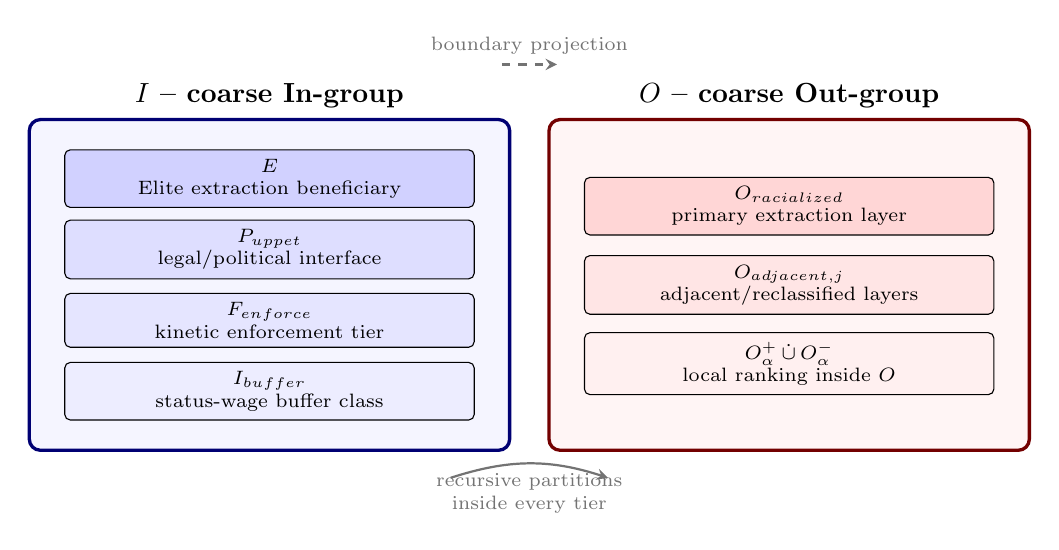
\begin{tikzpicture}[
    tier/.style={draw, rounded corners=2pt, align=center, font=\scriptsize, minimum height=0.62cm},
    bigbox/.style={draw, very thick, rounded corners=4pt, minimum height=4.2cm, minimum width=6.1cm},
    arr/.style={->, thick, >=stealth}
]
    \node[bigbox, fill=blue!4, draw=blue!45!black, label={[font=\bfseries]above:$I$ -- coarse In-group}] (Ibox) at (-3.3,0) {};
    \node[tier, fill=blue!18, minimum width=5.2cm] at (-3.3,1.35) {$E$\\Elite extraction beneficiary};
    \node[tier, fill=blue!13, minimum width=5.2cm] at (-3.3,0.45) {$P_{\text{uppet}}$\\legal/political interface};
    \node[tier, fill=blue!10, minimum width=5.2cm] at (-3.3,-0.45) {$F_{\text{enforce}}$\\kinetic enforcement tier};
    \node[tier, fill=blue!7, minimum width=5.2cm] at (-3.3,-1.35) {$I_{\text{buffer}}$\\status-wage buffer class};

    \node[bigbox, fill=red!4, draw=red!45!black, label={[font=\bfseries]above:$O$ -- coarse Out-group}] (Obox) at (3.3,0) {};
    \node[tier, fill=red!16, minimum width=5.2cm] at (3.3,1.0) {$O_{\text{racialized}}$\\primary extraction layer};
    \node[tier, fill=red!10, minimum width=5.2cm] at (3.3,0.0) {$O_{\text{adjacent},j}$\\adjacent/reclassified layers};
    \node[tier, fill=red!6, minimum width=5.2cm] at (3.3,-1.0) {$O^{+}_{\alpha} \,\dot\cup\, O^{-}_{\alpha}$\\local ranking inside $O$};

    \draw[arr, dashed, black!55] (-0.35,2.8) -- node[above, font=\scriptsize] {boundary projection} (0.35,2.8);
    \draw[arr, bend left=18, black!55] (-1.0,-2.45) to node[below, font=\scriptsize, align=center] {recursive partitions\\inside every tier} (1.0,-2.45);
\end{tikzpicture}
\caption{\textbf{Zooming the Binary.} The In-group/Out-group distinction remains the first projection, but higher resolution reveals internal tiers inside $I$, fractured layers inside $O$, and local In-group/Out-group relations inside each macro-class.}
\label{fig:binary-refinement}
\end{figure}

This refinement is why the framework can say two things at once without
contradiction: the In-group/Out-group model is correct at the first projection,
and it is insufficient as a full diagnostic. The deeper architecture appears
only after the binary is recursively resolved.



To develop and validate this framework, I examine \textbf{racism} as the primary case study---specifically, the American system of racial oppression from its colonial origins to the present. Racism provides an ideal test case because of its extensive historical documentation, its clear policy mechanisms, and its ongoing relevance. Through set-theoretic analysis, I demonstrate that racism exhibits all four architectural components and, in particular, that $O_{\text{racialized}}$ has \textit{expanded} over time.

This expansion reveals a deeper pattern: the Elite class ($E \subset I$) uses racial division to prevent cross-group solidarity and captures the surplus, while the racial In-group receives status wages and remains exploited. The ``public and psychological wage'' \cite{dubois, roediger}---Du Bois's term for the compound of status benefits and public infrastructure advantages granted to the buffer class $I \setminus E$---suppresses cross-class solidarity while $E$ extracts value from both groups. When status wages prove insufficient, material concessions are deployed, but always funded by deeper extraction from $O_{\text{racialized}}$: $\Delta\max = 0$ for $E$ is invariant.

Du Bois identified a second, equally critical mechanism in the final chapter of \textit{Black Reconstruction}---what he called the ``Propaganda of History'': the deliberate distortion of the historical record to erase Black agency, recast Reconstruction as a failure of Black governance, and naturalize the counter-revolution as inevitable restoration. This book treats the ``Propaganda of History'' as the first documented formal analysis of $P_{\text{gaslight}}$---the ideological variable that converts the extraction architecture into a self-concealing system. Du Bois showed that historiography itself can function as an enforcement mechanism: when the algorithm's own operations are written out of the record, each generation of potential resisters must rediscover the terrain from scratch. The diagnostic function of this book is, in part, a direct continuation of that anti-gaslighting project; see Section~\ref{sec:gaslighting} for the full formalization.

The architecture of this system---which I formalize as a Predatory Min-Max Function optimizing Elite extraction against class resistance---operates through recognizable patterns that can be formalized, identified, and resisted across contexts.

\textbf{A critical methodological note}: Comparing the \textit{architecture} of different oppressive systems is distinct from comparing their \textit{phenomenology}. This book analyzes design principles---how asymmetry is created, justified, and maintained. It does not measure magnitudes of suffering. Recognizing shared structure illuminates how systems of domination reproduce themselves and preserves the unique gravity of each manifestation.

\section{Racism as Primary Example}

\textbf{The Problem with Traditional Definitions}

Traditional definitions of racism reveal a troubling pattern: they relegate the systemic dimension to secondary or tertiary status, often buried as the third or fourth definition in dictionaries---the ``cliff notes'' version that few people encounter or use. Consider typical definitional hierarchies:

\begin{enumerate}
    \item \textbf{Primary definition}: Individual prejudice or discrimination based on race
    \item \textbf{Secondary definition}: Belief in racial superiority
    \item \textbf{Tertiary definition} (if present at all): Systemic or institutional discrimination
\end{enumerate}

This ordering reverses the causal structure. By centering individual prejudice, these definitions obscure the cardinal reality: \textit{the systemic element is the primary operation}. The interpersonal manifestations---individual prejudice, discriminatory actions, racial animus---are \textit{downstream products} created to maintain the systemic structure.

\textbf{Reversing the Causal Arrow}

The conventional framing suggests this causal relationship:
\begin{equation}\label{eq:1.3-conventional-causal-arrow}
\text{Individual Prejudice} \rightarrow \text{Discriminatory Actions} \rightarrow \text{Systemic Outcomes}
\end{equation}

This\footnote{This equation is classified as Tier~3 (ordinal/structural); the conventional causal arrow is a structural claim whose \textit{inversion} is validated by the historical sequence of deliberate Elite design documented in Chapter~\ref{ch:portugal} (p.~\pageref{ch:portugal}). See the Empirical Methodology chapter (p.~\pageref{ch:empirical_methodology}) and Appendix~\ref{app:empirical_index}.} implies that if we eliminate individual prejudice, systemic racism will disappear. History reveals the opposite causal structure:
\begin{equation}\label{eq:1.4-elite-causal-arrow}
\text{Elite Economic Interests} \rightarrow \text{Systemic Racialization} \rightarrow \text{Interpersonal Prejudice}
\end{equation}

As\footnote{This equation is classified as Tier~3 (ordinal/structural); the correct causal ordering---Elite economic interest preceding and producing interpersonal prejudice---is a structural claim validated by the documented historical sequence of Zurara's commissioned dehumanization (1453) and the \textit{Casa dos Escravos} (1486) narrated in Chapter~\ref{ch:portugal}. See the Empirical Methodology chapter (p.~\pageref{ch:empirical_methodology}) and Appendix~\ref{app:empirical_index}.} demonstrated in Chapter~\ref{ch:portugal}, interpersonal racism---the attitudes, beliefs, and prejudices held by individuals---\textit{was deliberately created to justify and maintain the systemic structure}. Zurara's racialization of Africans as subhuman was commissioned work designed to justify a system of unlimited exploitation \cite{zurara, biewen}. It was not a spontaneous expression of Portuguese prejudice. The systemic preceded the interpersonal (see Figure~\ref{fig:causal_reversal}).

\begin{figure}[htbp]
\centering
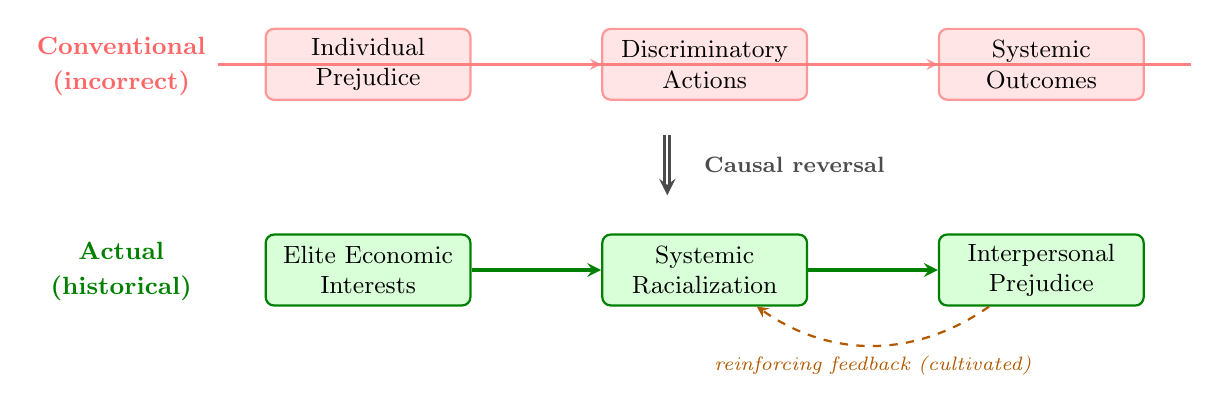
\begin{tikzpicture}[
    box/.style={draw, thick, rounded corners=3pt, minimum height=0.9cm, minimum width=2.6cm, align=center, font=\small},
    arr/.style={->, thick, >=stealth},
    scale=0.95
]
    % --- Conventional (incorrect) row ---
    \node[font=\small\bfseries, red!60] at (-5.8,1.5) {Conventional};
    \node[font=\small\bfseries, red!60] at (-5.8,1.0) {(incorrect)};
    \node[box, fill=red!10, draw=red!40] (a1) at (-2.5,1.25) {Individual\\Prejudice};
    \node[box, fill=red!10, draw=red!40] (a2) at (2,1.25) {Discriminatory\\Actions};
    \node[box, fill=red!10, draw=red!40] (a3) at (6.5,1.25) {Systemic\\Outcomes};
    \draw[arr, red!40] (a1) -- (a2);
    \draw[arr, red!40] (a2) -- (a3);
    % Strike-through
    \draw[very thick, red!50] (-4.5,1.25) -- (8.5,1.25);

    % --- Reversal arrow ---
    \draw[arr, very thick, black!70, double] (1.5,0.3) -- (1.5,-0.5);
    \node[font=\footnotesize\bfseries, black!70] at (3.2,-0.1) {Causal reversal};

    % --- Correct row ---
    \node[font=\small\bfseries, green!50!black] at (-5.8,-1.25) {Actual};
    \node[font=\small\bfseries, green!50!black] at (-5.8,-1.75) {(historical)};
    \node[box, fill=green!15, draw=green!50!black] (b1) at (-2.5,-1.5) {Elite Economic\\Interests};
    \node[box, fill=green!15, draw=green!50!black] (b2) at (2,-1.5) {Systemic\\Racialization};
    \node[box, fill=green!15, draw=green!50!black] (b3) at (6.5,-1.5) {Interpersonal\\Prejudice};
    \draw[arr, green!50!black, very thick] (b1) -- (b2);
    \draw[arr, green!50!black, very thick] (b2) -- (b3);
    % Reinforcing feedback loop (cultivated by the system)
    \draw[arr, orange!70!black, thick, dashed] (b3) to[bend left=35] node[below, font=\scriptsize\itshape, text=orange!70!black, pos=0.5] {reinforcing feedback (cultivated)} (b2);
\end{tikzpicture}
\caption{\textbf{The Causal Reversal with Reinforcing Feedback.} The conventional framing (top, struck through) assumes individual prejudice produces systemic outcomes. The historical evidence (bottom) reveals the opposite: Elite economic interests created systemic racialization, which then cultivated interpersonal prejudice to maintain the structure. The dashed feedback arrow acknowledges that interpersonal prejudice does reinforce systemic outcomes---but this loop is itself a product of the system's design, not its origin.}
\label{fig:causal_reversal}
\end{figure}

\paragraph{The feedback loop: bidirectional reinforcement within a primary causal direction.}
A precise framework must acknowledge what a simplistic unidirectional claim would obscure: interpersonal prejudice, once cultivated, \textit{does} feed back into systemic outcomes. A hiring manager's implicit bias reduces Out-group employment; a jury's racial priors produce harsher sentences; a voter's racial resentment elects $P_{\text{uppet}}$ candidates who expand the carceral state. These are real causal pathways from interpersonal attitudes to systemic outcomes. The framework does not deny them.

What the framework establishes is the \textbf{asymmetry of the causal relationship} and the \textbf{origin of the feedback loop itself}. The primary arrow---Elite economic interests $\rightarrow$ systemic racialization $\rightarrow$ interpersonal prejudice---is the \textit{generative} direction: without it, the feedback loop does not exist. Ambient phenotypic prejudice circulated in the medieval Mediterranean long before 1453, operating as a negotiable cultural attitude---a scalar carrying emotional magnitude without institutional direction \cite{sweet_iberian_roots_1997,bethencourt_racisms_2013}. Zurara's commissioned text marks the point where that ambient prejudice was systematized, legally codified, and structurally leveraged into an extraction architecture; Chapter~\ref{ch:portugal} documents this as the zero-day exploit. The generative claim is therefore precise: the system recruited pre-existing bias and manufactured its durable, heritable, self-replicating institutional form \textit{to serve} the systemic architecture. The reverse arrow---interpersonal prejudice reinforcing systemic outcomes---is a \textbf{maintenance loop}; it is not the causal origin. And critically, this maintenance loop constitutes a \textit{designed feature}: the Bayesian defense (Section~1.2.2), the corrupted firewall (Section~1.3.3), and the phase-loading architecture (Section~\ref{sec:phase_loading_algebra}) are all mechanisms by which the system deliberately cultivates and amplifies the very interpersonal attitudes that reinforce it. The system breeds its own antibodies.

This distinction has direct policy implications. Interventions targeting interpersonal prejudice---implicit bias training, diversity education, representation campaigns---address the \textit{feedback loop} without reaching the \textit{generative architecture}. They can reduce the loop's amplitude without touching the primary causal arrow. This is why such interventions produce measurable but limited effects: they attenuate a reinforcing signal without altering the kernel that produces it. The framework predicts that lasting structural change requires intervention at the generative level---the economic and political architecture that creates the conditions under which prejudice becomes rational self-interest for the Buffer Class.

\textbf{The Linguistic Evidence}

Moreover, traditional definitions overlook a fundamental linguistic aspect: the suffix ``-ism'' in ``racism'' already denotes a \textit{system}. We recognize this in other contexts:
\begin{itemize}
    \item \textbf{Capitalism}: A \textit{system} of economic organization, exceeding individual acts of trade
    \item \textbf{Feudalism}: A \textit{system} of social hierarchy, exceeding individual lord-serf relationships
    \item \textbf{Colonialism}: A \textit{system} of territorial exploitation, exceeding individual acts of conquest
\end{itemize}

With racism, we persistently treat it as a collection of individual attitudes, ignoring the systemic nature embedded in the structure of the word. That misreading serves a function: it deflects attention from the structural mechanisms that create and perpetuate racial inequality.

\textbf{The Critical Distinction: Racism and Prejudice Are Different Phenomena}

This analysis reveals a fundamental conceptual error in conflating racism with prejudice or bias. The distinction is categorical:

\begin{quote}
\textbf{Prejudice or bias}: Individual attitudes, stereotypes, or discriminatory behaviors based on group membership. These are interpersonal phenomena that can exist in any direction and between any groups.

\textbf{Racism}: A \textit{system of oppression} that weaponizes prejudice and bias into structural mechanisms of exploitation and control. Racism takes individual prejudice and transforms it through institutionalization into a self-perpetuating apparatus that serves Elite economic interests.
\end{quote}

\textbf{The systemic element distinguishes racism from prejudice.} The system is the \textit{defining characteristic} that separates racism from generic bias. Consider:

\begin{itemize}
    \item A person holding negative stereotypes about another group = \textbf{prejudice}
    \item A system that codifies those stereotypes into law, policy, and institutional practice to extract labor and prevent solidarity = \textbf{racism}
\end{itemize}

Racism is the process of taking interpersonal prejudice and bias---which exist across all human societies---and \textbf{weaponizing them} into a system that:
\begin{enumerate}
    \item \textbf{Institutionalizes} prejudice through policy ($P$)
    \item \textbf{Concentrates} harm at the intersection $O_{\text{racialized}} \cap P$
    \item \textbf{Naturalizes} the resulting disparities through ideology
    \item \textbf{Compounds} disadvantage over time through the mechanisms described in Chapter~\ref{ch:enforcement}
    \item \textbf{Serves} Elite economic interests by preventing working-class solidarity
\end{enumerate}

This distinction has significant implications. An individual can hold prejudices without participating in racism if those prejudices are not institutionalized into systems of power. Conversely, an individual can participate in and benefit from racist systems even while holding no conscious prejudice---because racism operates \textit{systemically}, through policies and structures, exceeding the scope of individual attitudes.

The conflation of racism with prejudice is imprecise and \textbf{functionally useful to the system}. By treating them as synonymous, we:
\begin{itemize}
    \item Suggest that eliminating individual prejudice eliminates racism
    \item Enable individuals to disavow racism by disavowing prejudice
    \item Obscure the structural mechanisms that create and maintain racial hierarchy
    \item Deflect attention from the Elite class that benefits from racial division
    \item Make structural analysis seem like an overreaction to individual attitudes
\end{itemize}

The system is \textit{the point}. Racism is fundamentally and irreducibly systemic. Prejudice, bias, and discrimination are real phenomena, but they are categorically different from racism as a system of oppression.

\textbf{Why the Misdirection Matters}

Centering individual prejudice as the primary definition of racism accomplishes several functions that protect the systemic structure:

\begin{enumerate}
    \item \textbf{Individualizes responsibility}: If racism is primarily individual prejudice, then solutions focus on changing hearts and minds and leave structures intact.
    
    \item \textbf{Obscures Elite benefits}: Individual-focused definitions hide the fact that racism serves Elite economic interests by preventing working-class solidarity.
    
    \item \textbf{Enables plausible deniability}: Individuals can claim ``I'm not racist'' (meaning ``I don't hold personal prejudice'') while participating in and benefiting from racist systems.
    
    \item \textbf{Makes structural critique seem extreme}: If racism is ``just'' individual prejudice, then analyzing systemic structures appears to be overreach or ``seeing racism everywhere.''
    
    \item \textbf{Perpetuates the system}: By misidentifying the disease (treating symptoms and leaving the cause intact), individual-focused definitions ensure the system persists.
\end{enumerate}

\textbf{The Correct Hierarchy}

A proper definition must reverse the conventional ordering, placing systemic policies at the center (see Figure~\ref{fig:hierarchy_inversion}):

\begin{enumerate}
    \item \textbf{Primary}: Racism is a \textit{system} of policies and structures that create and maintain racial hierarchies for Elite economic benefit
    \item \textbf{Secondary}: This system is justified through ideological narratives that naturalize racial categories and hierarchies
    \item \textbf{Tertiary}: These narratives manifest in interpersonal prejudices and discriminatory actions that reinforce the system
\end{enumerate}

This ordering reflects the historical reality established in Chapter~\ref{ch:portugal}: systemic racialization came first, ideological justification followed, and interpersonal prejudice was cultivated to maintain the structure. The interpersonal is real and harmful, but it is \textit{epiphenomenal}---a surface manifestation of the deeper systemic operation.

\begin{figure}[htbp]
\centering
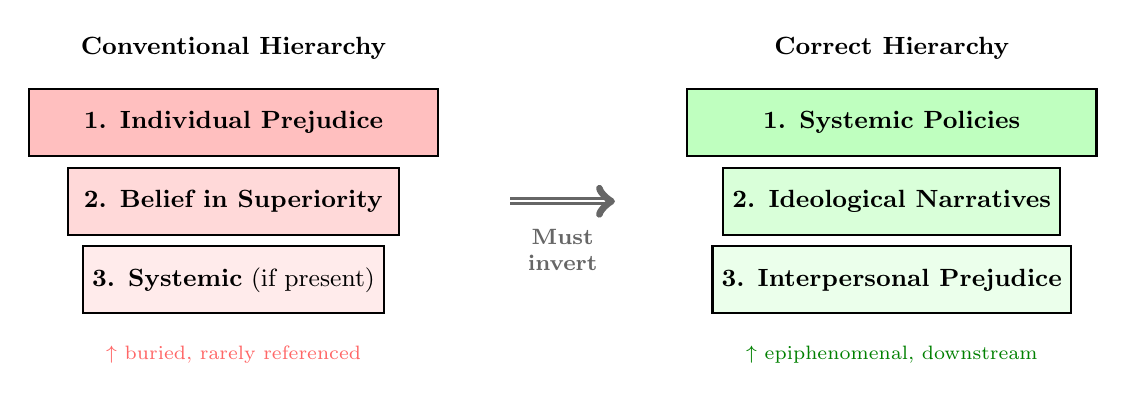
\begin{tikzpicture}[
    layer/.style={draw, thick, minimum width=4.8cm, minimum height=0.85cm, align=center, font=\small},
    scale=0.95
]
    % --- Conventional (left) ---
    \node[font=\small\bfseries] at (-3.5,3.2) {Conventional Hierarchy};
    % Primary (largest, top)
    \node[layer, fill=red!25, minimum width=5.2cm] (c1) at (-3.5,2.2) {\textbf{1. Individual Prejudice}};
    \node[layer, fill=red!15, minimum width=4.2cm] (c2) at (-3.5,1.15) {\textbf{2. Belief in Superiority}};
    \node[layer, fill=red!8, minimum width=3.2cm] (c3) at (-3.5,0.1) {\textbf{3. Systemic} (if present)};
    \node[font=\scriptsize, red!60] at (-3.5,-0.9) {$\uparrow$ buried, rarely referenced};

    % --- Arrow between ---
    \draw[->, very thick, black!60, double] (0.2,1.15) -- (1.6,1.15);
    \node[font=\footnotesize\bfseries, black!60, align=center] at (0.9,0.5) {Must\\invert};

    % --- Correct (right) ---
    \node[font=\small\bfseries] at (5.3,3.2) {Correct Hierarchy};
    % Primary (largest, top)
    \node[layer, fill=green!25, minimum width=5.2cm] (r1) at (5.3,2.2) {\textbf{1. Systemic Policies}};
    \node[layer, fill=green!15, minimum width=4.2cm] (r2) at (5.3,1.15) {\textbf{2. Ideological Narratives}};
    \node[layer, fill=green!8, minimum width=3.2cm] (r3) at (5.3,0.1) {\textbf{3. Interpersonal Prejudice}};
    \node[font=\scriptsize, green!50!black] at (5.3,-0.9) {$\uparrow$ epiphenomenal, downstream};
\end{tikzpicture}
\caption{\textbf{Inverting the Definitional Hierarchy.} Conventional definitions (left) bury the systemic dimension as a tertiary afterthought. The correct hierarchy (right) places systemic policies at the top, recognizing that ideological narratives and interpersonal prejudice are downstream products of the system.}
\label{fig:hierarchy_inversion}
\end{figure}

To address this fundamental gap in conventional definitions, I propose a new definition that places the systemic element where it belongs: at the center of analysis. This definition emphasizes racism as a system of oppression, deeply rooted in historical practices and policies that categorize individuals based on perceived racial differences---a system deliberately created by Elites to break class solidarity and maintain exploitable labor.

\section{The Diagnostic Model: Racism as a Fractal Computer Virus}

The definitional framework above establishes \textit{what} racism is. Before proceeding to the historical timeline, we require a diagnostic model that captures \textit{how it operates}: as a dynamic, adaptive, self-replicating system. The most precise analogue is computational. Systemic racism behaves exactly like a \textbf{fractal computer virus}: unauthorized code that hijacks a system's resources to execute its own programming, replicates itself across every scale of the network, and mutates its signature to evade detection---while its core payload never changes.

The virus frame is a \textit{diagnostic model}, not rhetorical decoration. Every component of the virus architecture corresponds to a variable or mechanism documented in the chapters that follow. The reader who holds this model in mind will recognize each historical episode as a specific module of the same malicious code executing across five centuries.

From the host side, the same architecture is the \textbf{fractal mind virus}: the institutional exploit becomes durable only when it can run on ordinary human cognition. Law supplies the executable file; schools, churches, newspapers, courts, parties, and police supply the update channels; the brain's inherited shortcuts supply the vulnerable wetware. The diagnostic question in every chapter is therefore twofold: ``What policy was passed?'' and ``What prior did that policy install in the population that made the next policy feel natural?''

\begin{definition}[Biological Embedding]
\label{def:biological_embedding}
\textbf{Biological embedding} names the process by which chronic social exposure
becomes physiological system state. In this framework, racism does not become
biological because race is genetic, and it does not transmit moral essence
through blood. It becomes biological because law, policing, poverty, spatial
containment, humiliation, and anticipatory threat repeatedly activate stress
pathways until the body carries the history as allostatic load, inflammation,
telomere shortening, DNA-methylation changes, accelerated epigenetic aging, and
altered threat calibration. The claim is therefore bounded: the extraction
system can write itself into bodies without making the hierarchy natural.
\end{definition}

This evidence boundary is essential. Human studies support biological embedding
and intergenerational stress effects, but they do not justify claims that cruelty
or innocence is genetically inherited. The strongest race-specific evidence in
this book therefore concerns weathering, allostatic load, inflammation, telomere
length, and methylation patterns under repeated discrimination
\cite{geronimus_weathering_2006,duru_allostatic_mortality_2012,ruiz_narvaez_racism_methylation_2024,spears_lifespan_stress_inflammation_2026}.
Human intergenerational epigenetic evidence remains more cautious: famine,
Holocaust, and Civil War POW studies show plausible mechanisms and persistent
marks or downstream outcomes, but reviews emphasize small samples, confounding,
and the difficulty of separating germline inheritance from prenatal exposure,
caregiving, material deprivation, and social transmission
\cite{heijmans_dutch_famine_methylation_2008,yehuda_holocaust_fkbp5_2016,costa_paternal_trauma_pow_2018,zhou_ryan_biological_embedding_2023}.

The empirical anchors used throughout the book are embedded as module tests in each chapter. Each source below validates one runtime layer of the same exploit while leaving the book's formal interpretation to do the synthetic work:

\begin{center}
\renewcommand{\arraystretch}{1.25}
\begin{tabular}{>{\raggedright}p{3.0cm} >{\raggedright}p{3.2cm} >{\raggedright\arraybackslash}p{7.6cm}}
\toprule
\textbf{Runtime layer} & \textbf{Framework variables} & \textbf{Empirical anchor} \\
\midrule
Spatial infrastructure & $P_{\text{spatial}}$, $\Sigma_{\text{sup}}$ & Covenants, lending, redlining, and firearm-violence studies show containment operating through interoperable public and private nodes, not through one federal lever \cite{toney_housing_covenants_2026,barboza_salerno_redlining_firearm_2025}. \\
Judicial software & $P_{\text{jud}}$ & Text-based and expert-sourced ideology measures support treating judicial language as observable evidence of latent preference weights, exceeding neutral doctrine \cite{truscott_romano_judicial_text_2026,cope_judjis_2025}. \\
Carceral firewall & $P_{\text{carceral}}$ & Pretrial incarceration functions as political deletion before conviction, depressing turnout through a facially procedural criminal-legal interface \cite{enamorado_shadow_carceral_2024}. \\
Physical output & $P_{\text{lead}}$, $\Sigma_{\text{sup}}$, $\tau$ & Lead exposure and child-mortality frontier studies show how spatial inequality becomes biological depletion and mortality risk at the boundary of concentrated hardship \cite{berisha_lindstrom_kosovo_roma_2024,barboza_salerno_child_frontiers_2025}. \\
Embodied runtime & $\Delta(t)$, $\Pi_{\text{race}}$, $O_{\text{racialized}}$ & Weathering, allostatic load, inflammation, telomere, and methylation studies show that chronic racialized stress can become biological system memory without implying genetic race or inherited moral essence \cite{geronimus_weathering_2006,ruiz_narvaez_racism_methylation_2024,spears_lifespan_stress_inflammation_2026}. \\
\bottomrule
\end{tabular}
\end{center}

\subsection{Canonical Variable Map: Kernel Semantics and Dynamic State}

To keep the formal system coherent across chapters, we use a dual map: kernel semantics (\texttt{Max/Min}) and dynamic state variables ($\mathcal{E}(t)$/$M(t)$).

\begin{center}
\renewcommand{\arraystretch}{1.35}
\begin{tabular}{>{\raggedright}p{3.3cm} >{\raggedright}p{3.4cm} >{\raggedright\arraybackslash}p{7.4cm}}
\toprule
\textbf{Kernel Semantic} & \textbf{Dynamic Symbol} & \textbf{Meaning} \\
\midrule
Extraction objective & $\mathcal{E}(t)$ & Time-indexed extraction output (material transfer toward $E$). \\
Resistance control & $M(t)$ & Time-indexed class-coherence threat (dynamic analogue of $\min$-management pressure). \\
Collapse threshold & $\tau$ & Critical coherence threshold where the kernel destabilizes. \\
Suppression allocation & $\psi(t) = \psi_s(t) + \psi_m(t)$ & Two-mode compensation to $I_{\text{buffer}}$: $\psi_s$ (status/symbolic, always active) and $\psi_m$ (material concession, deployed when $M(t) \to \tau$; sourced from $O_{\text{racialized}}$ extraction). \\
Kinetic repression & $R(t)$ & Physical suppression capacity of $F_{\text{enforce}}$. \\
Phase architecture & $\phi_{k,j}, \Phi_j$ & Axis-level and compound phase shifts that fragment class-alignment waves. \\
\bottomrule
\end{tabular}
\end{center}

\textbf{Notation rule}: $E$ denotes the Elite class set exclusively; $\mathcal{E}(t)$ denotes the time-indexed extraction output function. $\mathcal{S}_{\text{enc}}$ denotes the Enclosure Score (Tri-Modal Enclosure Model, Section~\ref{sec:trimodal}). $\psi$ is reserved exclusively for psychological wage. Phase variables use only $\phi/\Phi$ notation. Symbol reuse is disallowed.

\subsection{The Core Payload: A Resource-Mining Rootkit}

The primary objective of a computer virus is usually hidden from the user. The system appears to function normally; the extraction occurs in the background.

In this framework, the racial hierarchy functions as a highly successful \textbf{resource-mining rootkit} installed by the Elite ($E$) inside the American operating system. Its singular function is to hijack the system's processing power---human labor, human time, human bodies---to indefinitely mine wealth for the system's administrators. This is the $\max$ variable of the Predatory Min-Max Function: the uninterrupted flow of extracted value from the population to the Elite.

Formally, the kernel objective is:
\begin{equation}\label{eq:1.5-kernel-optimization}
\max \mathcal{E}(t) \quad \text{subject to} \quad M(t) < \tau
\end{equation}
where $M(t)$ is class-coherence risk (the dynamic analogue of the $\min$ stress variable) and $\tau$ is the crash threshold.

\paragraph{The minimum forcing threshold.}
The Declaration of Independence supplied the political vocabulary for this threshold before the framework supplied the notation. Jefferson's ``long train of abuses and usurpations'' names a cumulative forcing condition \cite{declaration_independence_1776}. A population crosses the kinetic boundary when repeated extraction compounds past the point where continued compliance is less rational than structural rupture:
\begin{equation}\label{eq:1.5a-minimum-forcing-threshold}
\mathcal{A}_{\text{abuse}}(t)
=
\int_{0}^{t} \mathcal{E}_{\max}(s)\,ds
\quad \text{and breach occurs when} \quad
\mathcal{A}_{\text{abuse}}(t) \geq \tau_{\text{MFT}} .
\end{equation}
The minimum forcing threshold ($\tau_{\text{MFT}}$) is therefore the temporal form of $\tau$: it measures accumulated extraction, humiliation, enclosure, and failed remedy over time. This matters because the algorithm's most dangerous phase is the long period in which brutality is normalized, routed through proxy variables, and compounded until the threshold has already been crossed before the governing class recognizes it.

The rootkit hides deep in the operating system's \textbf{kernel}---the Constitution, the early property laws, the 13th Amendment's exception clause. Standard user-level actions (voting, protesting, filing lawsuits, electing sympathetic candidates) cannot access, modify, or delete code running at the kernel level. The model therefore predicts that user-space reforms cannot interrupt kernel-level extraction---and the chapters that follow confirm this: every major non-kinetic reform examined in this study was absorbed by the algorithm without altering $\max$. The extraction payload has been running since 1619, and no user-level intervention in the historical dataset has interrupted it.

The formal containment model of Section~\ref{sec:formal-containment-model} gives this non-responsiveness a precise meaning. $E$ is defined as the set of \textbf{stationary leaders}: agents whose state obeys ${}_{\,0}D_t^{\alpha} q_i(t) = 0$, i.e., whose dynamics do not admit a user input $u_i$. Every follower equation contains $u_i$; the leader equations do not. The claim ``user-level reforms cannot touch the kernel'' is, in that framework, a trivial consequence of which equations the control input appears in.\footnote{The sequence of version-update runtime logs that open each chapter---1486 (Lisbon), 1676 (Bacon's Rebellion), 1705 (Virginia Slave Codes), 1787 (Constitutional Convention), 1803 (Louisiana Purchase), 1865 (13th Amendment), 1894--1934 (Pullman/Redlining), 1964--1968 (Civil Rights/War on Drugs), 1994 (Crime Bill)---corresponds structurally to what Acemoglu and Robinson term ``critical junctures'' in \textit{Why Nations Fail} \cite{acemoglu_robinson}: historical moments at which the balance of institutional power shifts, making some trajectories available and others foreclosed. The framework's version-update model operationalizes the critical-juncture concept: each runtime log is a moment when the Elite ($E$) detected a $\min$-failure threat, assessed the cost function of available interface strategies ($S^\ast(t)$), and recompiled the extraction kernel with a new interface. AJR identify these moments; the Predatory Min-Max Function specifies the optimization logic that selects among available responses.}

\subsection*{Case Study: Kernel Optimization in the Antebellum South, 1840--1860}
\label{cs:kernel_antebellum}

\paragraph{Setup.}
The antebellum cotton economy (1840--1860) constitutes the most fully documented instantiation of the kernel objective defined in Equation~\ref{eq:1.5-kernel-optimization}. During this period, the extraction variable $\mathcal{E}(t)$---operationalized as total annual cotton revenue---grew by more than 230\% in nominal terms across three decennial Census intervals. This growth was the direct output of a system optimizing extraction at scale, deploying enslaved labor as capital and land as infrastructure. The framework's prediction is precise: as $\mathcal{E}(t)$ increases, the kernel must proportionally scale suppression expenditure to keep class-coherence risk $M(t)$ below the crash threshold $\tau$. A kernel that extracts without maintaining the suppression constraint will breach $M(t) = \tau$ and collapse.

\paragraph{Data sources.}
Cotton output and revenue data are drawn from the U.S. Census Bureau's \textit{Historical Statistics of the United States, Colonial Times to 1970}, Series~K~554--563 \cite{census_hist_stats}. Slave population figures are from the 1840, 1850, and 1860 decennial Census schedules \cite{census_1860}. Militia and slave patrol expenditure estimates are compiled from state legislative appropriations records documented in Hadden's \textit{Slave Patrols} \cite{hadden_slave_patrols} and corroborated against the broader economic histories in Beckert's \textit{Empire of Cotton} \cite{beckert} and Baptist's \textit{The Half Has Never Been Told} \cite{baptist}. Curated data are archived at \texttt{Paper/data/eq05\_antebellum\_cotton.csv}; computational results are reproducible via \texttt{Paper/scripts/eq05\_kernel\_optimization.ipynb}.

\paragraph{Operationalization.}
The equation's three variables are mapped to historical observables as follows. $\max \mathcal{E}(t)$ is operationalized as annual cotton revenue in U.S. dollars---the principal extraction output of the antebellum kernel. $M(t)$ (class-coherence risk) is operationalized as the \textit{suppression budget ratio}: militia and slave patrol expenditure as a fraction of total cotton revenue. A stable or proportionally growing ratio signals that the Elite is actively maintaining $M(t) < \tau$ by scaling enforcement with extraction; a declining ratio would signal extraction without commensurate suppression investment. $\tau$ is the crash threshold: the point at which class-coherence risk exceeds the system's containment capacity, as observed empirically in events like Nat Turner's Rebellion (1831) and, ultimately, the Civil War.

\paragraph{Numerical computation.}
The notebook computes the suppression budget ratio for the 1840, 1850, and 1860 Census intervals. Results are as follows: in 1840, cotton revenue stood at approximately \$74.1M against militia/patrol expenditure of approximately \$2.0M, yielding a suppression ratio of 2.70\%. In 1850, revenue had grown to \$102.5M with expenditure of \$2.95M (ratio: 2.88\%). By 1860, revenue reached approximately \$247.0M while suppression expenditure scaled to approximately \$6.8M (ratio: 2.75\%). Across a period in which extraction tripled, the suppression ratio varied within a band of less than 0.2 percentage points---a coefficient of variation below 0.04. The slave population grew from 2,487,455 in 1840 to 3,953,761 in 1860, reflecting the simultaneous expansion of the extraction base.

\begin{figure}[htbp]
  \centering
  
\includegraphics[width=\textwidth]{figures/eq05_kernel_optimization.png}
  \caption{Kernel optimization in the Antebellum South, 1840--1860. Left axis: cotton revenue (millions USD). Right axis: suppression budget ratio (\%). Despite a 233\% increase in extraction revenue, the suppression ratio held within a 0.18 percentage-point band (CV $<$ 0.04), confirming proportional enforcement scaling as predicted by eq.~\ref{eq:1.5-kernel-optimization}.}
  \label{fig:eq05_kernel}
\end{figure}

\paragraph{Comparison to prediction.}
Equation~\ref{eq:1.5-kernel-optimization} predicts that a kernel maximizing $\mathcal{E}(t)$ subject to $M(t) < \tau$ will scale enforcement expenditure proportionally with extraction output---not allow enforcement to lag. The data confirm this prediction at every Census interval: the suppression ratio remained within a tightly controlled band even as nominal extraction tripled. This is precisely the optimization signature the equation describes: the kernel does not extract and then suppress reactively; it maintains suppression capacity as a fixed constraint on extraction expansion. Beckert and Baptist independently document the institutional mechanisms---the expansion of the slave patrol system, the legal deputization of the entire white male population, and the passage of increasingly severe fugitive slave legislation---that operationalized this proportional scaling.

\paragraph{Precision qualifier: the cotton gin as a confound.}
The anticipated objection is that cotton revenue and suppression spending grew together solely because Eli Whitney's cotton gin (1793) drove a technology-led boom---an economic growth story, not an optimization story. This objection fails on three grounds. First, the gin reduced the labor cost of \textit{processing} cotton fiber but made cultivation so profitable that planters massively expanded acreage, requiring \textit{more} enslaved labor, not less: the enslaved population grew from approximately 700,000 in 1790 to 3,953,761 by 1860. The gin expanded the extraction base without reducing the need for suppression. Second, a pure technology-efficiency story predicts a \textit{declining} suppression ratio---higher output per worker should mean lower rebellion risk per unit of extraction. The data show the opposite: the ratio held constant within a 0.18 percentage-point band across the gin era's revenue tripling. Third, the gin is itself an instance of the kernel objective in action: when a technology became available that increased $\mathcal{E}(t)$, the Elite deployed it. The kernel's adoption of a more efficient extraction mechanism confirms eq.~\ref{eq:1.5-kernel-optimization}; it does not refute it. The constraint $M(t) < \tau$ then required suppression to scale with the expanded enslaved population, which it did. The Nat Turner Rebellion (August 1831, between the 1820 and 1840 Census intervals) provides an independent within-period falsification test: when class-coherence risk spiked, the immediate legislative response across the South was a dramatic tightening of slave codes---a documented $\tau$-management response that the cotton gin cannot explain and the optimization model predicts directly.

\paragraph{Falsification criteria.}
This equation would be falsified if the historical record showed a sustained period (multiple consecutive years or Census intervals) in which cotton revenue increased while militia and slave patrol expenditure decreased or remained flat in nominal terms---i.e., if the kernel extracted without maintaining the suppression constraint. No such period is present in the data. The closest counterfactual---the post-1861 Union blockade, which disrupted cotton revenue while Confederate states \textit{increased} military expenditure to maintain $M(t) < \tau$ under existential threat---actually reinforces the prediction: even when extraction was interrupted, the suppression constraint remained the priority.

\paragraph{Confidence tier.}
\textbf{Tier~1.} Three Census-year data points with direct correspondence between extraction output and suppression expenditure; corroborated by independent historical scholarship from Beckert, Baptist, and Hadden.

\subsection{The Zero-Day Exploit: The Invention of Race}

In cybersecurity, a \textbf{zero-day exploit} attacks a vulnerability that the system does not know it has. The target cannot defend against it because the vulnerability has not been identified, catalogued, or patched. It is the most dangerous class of attack precisely because the victim does not know they are vulnerable.

A precision note before proceeding: the zero-day was distinct from phenotypic \textit{awareness} itself. Phenotypic difference has been culturally marked since antiquity---ancient Greek and Roman writers noted skin color; Arab and Ottoman slave systems used phenotypic descriptors; African kingdoms traded enslaved persons across phenotypic lines. Grok and similar critics note this correctly, and the framework does not contest it. The zero-day exploit was the \textit{industrialization} of phenotype as a permanent, heritable, legally codified \textit{capital asset} at transatlantic scale. Earlier phenotypic prejudices existed as cultural attitudes that could be partially negotiated through religious conversion, geographic displacement, or social performance. Portugal's juridical and commercial apparatus invented the mechanism by which phenotype could be simultaneously embedded in property law, inheritance law, and international commodity markets---converting a soft cultural variable into a wetware-anchored legal partition that no amount of individual behavior could override. The zero-day was race written into code.

The Portuguese Elite discovered a zero-day exploit in human psychology: the capacity to partition populations into In-groups and Out-groups using \textit{phenotypic markers} as the sorting key. As Chapter~\ref{ch:portugal} will document, the Elite had previously attempted to exploit religious identity as a partition variable---the French Wars of Religion (1562--1598) and the Thirty Years' War (1618--1648) killed millions using $J_{\text{religious}}$ as the ideological interface. But religious identity was a \textit{soft partition}: it could be changed through conversion, blurred through intermarriage, and eroded through cohabitation. Portugal, moreover, was largely a single ethnic group sharing a single religion---the existing partition variables were unavailable.

The zero-day was the discovery that \textit{phenotype}---skin color, hair texture, facial features---could serve as a permanent, heritable, visually self-enforcing partition variable. Race, in this context, is primarily a phenotypic categorization based on superficial expressions like skin pigment; it does not rest on significant genetic difference beyond those expressions. In fact, the greatest human biodiversity is found on the African continent. Unlike religion, phenotype could not be changed through conversion. Unlike nationality, it could not be changed through migration. Unlike class, it could not be changed through economic mobility. The racial partition was a \textbf{wetware-level exploit}: it attacked the biological presentation layer of the human operating system, a layer that no amount of software updates (education, legislation, moral progress) could modify.

This zero-day was deployed at scale through the Transatlantic Slave Trade---the mass installation of the malware across the global network. The trade \textbf{networked global economies} into a massive \textbf{botnet} where millions of enslaved Africans were forced into processing power for the Elite's capitalist extraction engine. This was the \textbf{spatial mathematics of the Middle Passage}: human beings packed spoonways in feces, blood, and mucus, resulting in a 15\% mortality rate---nearly 2 million deaths during transport. The math was quite literally written in blood. Every plantation was a compromised node. Every colonial economy was a conscripted server. To enforce the \textbf{minimum resistance variable} ($\min$), the system required the constant application of naked instrumental force and torture. ``Autonomy restriction'' names a documented reality: an enslaver who, because a baby would not eat, boiled the infant's legs, tied a log to its neck, beat it to death, and forced the mother to throw the body overboard as a public spectacle of absolute dominance; the horrific ``Darby's dose'' recorded in Thomas Thistlewood's 14,000-page diary; and the routine transformation of terror into management technique. The botnet's output---sugar, tobacco, cotton, rice---was routed to the Elite's capital accumulation infrastructure in Lisbon, London, Amsterdam, and eventually Wall Street.

\subsection{The Bayesian Defense: Hardwiring the Priors}
\label{sec:bayesian_defense}

\paragraph{Host wetware.}
The virus model requires an explicit execution substrate. The extraction code does not run on abstract society alone; it runs on the most efficient known pattern-recognition wetware: the human brain. That wetware is optimized for fast prediction, energy conservation, and social coordination, not for perfect truth-tracking under adversarial input. Social Identity Theory identifies the ordinary tendency to sort social reality through In-group/Out-group categories \cite{tajfel_turner_intergroup_conflict_1979}; predictive-coding and free-energy accounts model perception as the continuous reduction of prediction error through top-down priors and incoming sensory data \cite{friston_free_energy_2010,clark_whatever_next_2013}. The framework rejects biological inevitability: the Elite's legal and social code exploited a general-purpose cognitive architecture by routing its prediction machinery through a legally enforced racial partition.

A wetware-level exploit is only effective if the system's software cannot identify and override it. To defend the racial partition, the Elite developed an epistemic architecture that functions as a \textbf{Bayesian defense}. In terms of predictive coding, the human brain is an inference engine that constantly applies ``priors''---learned assumptions and established rules---to interpret sensory data. The fractal virus of racism works by installing a high-precision, top-down prior that mandates the hierarchy. If $X$ denotes raw sensory input, $T$ denotes a threat/status interpretation, and $\Pi_{\text{race}}$ denotes the installed racial prior, then stereotypes function as compressed Bayesian priors:
\[
P_i(T \mid X, \Pi_{\text{race}}) \propto P(X \mid T)\,P_i(T \mid \Pi_{\text{race}}).
\]
The malicious input is the legal-social prior $\Pi_{\text{race}}$ assigned excessive precision by repeated institutional reinforcement, not the brain's inference machinery itself. Once installed, that prior can dominate the interpretation of $X$, allowing phenotype, name, neighborhood, or proxy status to override direct evidence and empathy.

Every interaction, every policy, and every media representation serves as a data point reinforcing this prior. The system ensures that the ``race'' interface is so heavily weighted that it overpowers raw sensory input. This is the neurobiological foundation of selective empathy: the brain's predictive coding filters out Out-group harm because the prior has already categorized it as irrelevant or natural. 

A Mode~2 observation is instructive here (see Section~\ref{sec:conspiracy_emergence} for the full typology). Empirical research documented that specific pharmacological interventions could temporarily downregulate the Default Mode Network---the neurological conductor that maintains established cognitive models---producing a state in which subjects could ``take an overly rigid conception apart and reassemble it'' \cite{ifas_1966}. The 1966 IFAS Protocol reported a 91\% success rate on intractable professional problems through this mechanism. Within months, California criminalized LSD; the federal Drug Abuse Control Amendments extended the prohibition nationally; the Controlled Substances Act of 1970 completed the scheduling architecture. The framework does not assign intent to any individual actor in this sequence---moral panic, political opportunism, and genuine public-safety concerns all contributed, and this is an overdetermined institutional outcome. What the framework observes is the \textbf{functional output}: the one documented pharmacological tool capable of relaxing rigid predictive priors was removed from the research environment for over half a century. Whether that removal constituted deliberate epistemic containment (Mode~3) or emergent institutional response (Mode~2) is an open question the framework flags but does not resolve. A population capable of relaxing its predictive priors is a population capable of perceiving the extraction kernel through the racial noise; the functional output of this institutional sequence, regardless of proximate cause at any node, was the restoration of epistemic enclosure.

\subsection{Polymorphic Code: The Interface Swap}

\textbf{Polymorphic viruses} constantly change their identifiable features---their code signature---to evade antivirus detection, while keeping their malicious payload \textit{exactly the same}. This is the computational equivalent of the \textbf{Interface Swap} documented throughout this book.

The system's most foundational interface swap was the creation of the ``gastronomic interface.'' As Woodard demonstrates through the work of antebellum physician Samuel A.~Cartwright, the extraction payload was actively disguised as an acquired, refined taste. By constructing the Black captive as an edible, infantile, and exotic commodity---what Cartwright termed the ``childlike Negro''---the system converted raw extraction appetite into an aesthetic ``taste'' for the Elite. Racism operates as a legal and physical partition whose cultural interface is a \textit{palate formation} that aestheticizes dominance \cite{cartwright_report, woodard_delectable}.

Every time the host system's antivirus catches up---every time a reform movement identifies and targets the current interface of the extraction kernel---the virus recognizes the threat and \textbf{recompiles its code}:

\begin{itemize}
    \item \texttt{Chattel\_Slavery.exe} is detected and quarantined by the 13th Amendment (1865). The virus instantly recompiles as \texttt{Convict\_Leasing.exe} and \texttt{Black\_Codes.exe}---same extraction payload, new file signature.

    \item \texttt{Jim\_Crow.exe} is detected by the Civil Rights Movement (1964--1965). The virus morphs into \texttt{War\_on\_Drugs.exe} and \texttt{Mass\_Incarceration.exe}---the Variable Swap documented in Chapter~\ref{ch:recompile} replaces the explicit racial interface with facially neutral proxy variables ($P_{\text{criminal}}$, $P_{\text{spatial}}$) while preserving the asymmetric extraction function.

    \item \texttt{Explicit\_Discrimination.exe} is flagged by \textit{Brown v.\ Board} and the Civil Rights Act. The virus recompiles as \texttt{Redlining.exe}, \texttt{Predatory\_Lending.exe}, and \texttt{Algorithmic\_Bias.exe}---each iteration more difficult to detect because the racial interface has been abstracted behind layers of facially neutral code.
\end{itemize}

The first recompile remains visible in the present tense. Texas prison farms preserve the 13th Amendment exception as an operating labor interface: the \textit{Texas Observer} reports that 24 Texas prison units still have agribusiness operations, nine of them on former plantation land, with incarcerated workers compelled to labor without pay \cite{texas_observer_prison_plantations_2024}. The kernel survived the legal patch and continued executing through a new file signature, even as the surface changed after 1865.

The underlying payload---$\max \mathcal{E} - \min(I_{\text{buffer}} \cup O_{\text{racialized}})$---has not changed since 1450. Only the \textit{file name} and \textit{user interface} have changed. This is why purely moral arguments against racism fail: you cannot defeat a polymorphic rootkit by politely asking it to stop recompiling. You cannot ``educate'' malware into deleting itself. And you cannot neutralize the extraction kernel by changing the desktop wallpaper---by installing a Black CEO, a diversity training module, or a sympathetic president over a system whose kernel-level code remains untouched.

The interface swap is an optimizer, not an improvisation. Let
\begin{equation}\label{eq:1.6-interface-strategy-set}
S \in \{\text{partition},\text{integration},\text{direct repression},\text{externalization}\}
\end{equation}
and\footnote{This equation is classified as Tier~3 (ordinal/structural); the four-element strategy set is a structural enumeration whose coverage is validated by the historical case sequence in Chapters~2--10 (15th-century partition, Reconstruction-era integration offers, Jim Crow direct repression, and War on Drugs externalization). See the Empirical Methodology chapter (p.~\pageref{ch:empirical_methodology}) and Appendix~\ref{app:empirical_index}.}
\begin{equation}\label{eq:1.7-interface-optimizer}
S^\ast(t) = \arg\min_{S} \left[C_{\text{coercive}}(S,t) + C_{\text{legitimacy}}(S,t) + C_{\text{economic}}(S,t)\right]
\end{equation}
subject to preserving the extraction objective and keeping $M(t)$ below $\tau$.

\paragraph{Cost function definitions.}
The three cost components correspond to real deliberative trade-offs documented in Elite planning across every historical era studied:

\begin{itemize}[leftmargin=*]
    \item $C_{\text{coercive}}(S,t)$: the operational cost of enforcing strategy $S$ at time $t$. This includes labor and infrastructure for $F_{\text{enforce}}$, the risk that enforcement actions generate solidarity (i.e., increase $M(t)$, not suppress it), and the probability of kinetic blowback that threatens $\tau$. High-visibility violence---lynchings, fire hoses, mass arrests---carries high $C_{\text{coercive}}$ because each instance risks radicalizing additional nodes of $I_{\text{buffer}}$ and $O_{\text{racialized}}$.

    \item $C_{\text{legitimacy}}(S,t)$: the ideological exposure cost of strategy $S$ at time $t$ --- the degree to which $S$ is legible as a racial hierarchy to domestic audiences, international observers, or the judicial system, risking constitutional challenges, diplomatic condemnation, or buffer class defection. This cost is time-dependent: $C_{\text{legitimacy}}(\text{Jim Crow}, t)$ was low in 1870 and high by 1960, as the Cold War made explicit racial apartheid a geopolitical liability.

    \item $C_{\text{economic}}(S,t)$: the direct expense and opportunity cost of strategy $S$ at time $t$, including capital investment in new enforcement infrastructure, drag on $\mathcal{E}(t)$ from market disruption, and the long-term cost of maintaining strategy $S$ against rising resistance.
\end{itemize}

\paragraph{Historical calibration: Jim Crow $\to$ War on Drugs.}
The transition from explicit racial segregation to the carceral proxy system provides the clearest observable calibration of the optimizer. By the mid-1950s, all three cost functions for \texttt{Jim\_Crow.exe} were rising simultaneously:

\begin{itemize}[leftmargin=*]
    \item $C_{\text{legitimacy}}$: rising sharply. NAACP litigation had begun dismantling the legal architecture; \textit{Brown v.\ Board} (1954) exposed the explicit partition to federal judicial scrutiny; Cold War competition with the Soviet Union made domestic racial apartheid an international embarrassment, as documented by the State Department's own foreign policy reports \cite{dudziak}.
    \item $C_{\text{coercive}}$: rising. The Civil Rights Movement's strategy of non-violent public confrontation was specifically engineered to maximize the legitimacy cost of enforcement---fire hoses and police dogs in Birmingham generated exactly the global condemnation that forced the Elite to act.
    \item $C_{\text{economic}}$: rising. International trade relationships and the postwar liberal consensus were creating market incentives for surface-level integration that explicit segregation resisted.
\end{itemize}

The optimizer selected \texttt{War\_on\_Drugs.exe}---this is $S^*(t)$ from Equation~\ref{eq:1.7-interface-optimizer} executing in real time---because all three costs dropped simultaneously at the point of swap. $C_{\text{legitimacy}}$ fell to near zero: facially neutral language (``criminal,'' ``drug offender'') carried no explicit racial classification and had already been validated by the \textit{Williams v.\ Mississippi} (1898) architecture. $C_{\text{coercive}}$ fell: the proxy variable $P_{\text{criminal}}$ allowed the existing carceral infrastructure to process pre-criminalized populations with bureaucratic efficiency, eliminating the need for constant active enforcement theater---what Dan Baum reports John Ehrlichman described in a 1994 interview as the ability to ``arrest their leaders, raid their homes, break up their meetings, and vilify them night after night on the evening news'' without the political cost of explicit racial targeting \cite{baum}. The quote is treated here as testimonial evidence, not as a formal policy memorandum: Ehrlichman's family and some Nixon-era defenders have disputed its reliability, while the downstream policy pattern is independently confirmed by the statutory and incarceration record. $C_{\text{economic}}$ rose temporarily (prison construction) but was offset by the creation of a carceral industry that itself became an extraction mechanism.

The operational sequence is the proxy playbook: association $\rightarrow$ criminalization $\rightarrow$ enforcement $\rightarrow$ media-legitimation. Lee Atwater's 1981 description of Southern Strategy abstraction supplies the political-language layer: explicit racial appeals become coded policy terms, then apparently neutral economic or public-order language whose effects remain racially structured \cite{atwater, lopez}. Drug policy supplied the enforcement layer. Caulkins and Chandler estimate that people incarcerated for drug-law violations rose from 38,680 in 1972 to 480,519 in 2002---a more than twelvefold increase \cite{caulkins_chandler_drug_incarceration}. The crack/powder cocaine regime then gave the proxy a precise statutory geometry: pre-Fair Sentencing Act federal thresholds assigned comparable mandatory-minimum exposure to five grams of crack cocaine and 500 grams of powder cocaine, encoding a 100:1 disparity into federal sentencing practice \cite{ussc_crack_retroactivity_2011}. The racialized enforcement pattern is likewise documented in the drug-arrest record: ACLU analyses find comparable marijuana use rates across Black and white populations but sharply disparate arrest exposure \cite{aclu2013, aclu2020}. This is exactly the variable swap predicted by the optimizer: the label changes from race to criminality, while the target geometry remains legible in outcomes.

The Broward County reverse-sting cases supply the extreme boundary condition. In \textit{State v.\ Williams}, the Florida Supreme Court held that the Broward Sheriff's Office illegally manufactured crack cocaine from seized powder cocaine, packaged it for reverse-sting use, and thereby violated due process when prosecutors charged buyers caught in the resulting operations \cite{state_v_williams_1993}. Three decades later, Broward prosecutors sought to clear as many as 2,600 records tied to the same police-made-crack operations \cite{ap_broward_crack_vacatur_2024}. This case collapses any comforting distinction between ``crime control'' and crime production: under the proxy regime, $P_{\text{criminal}}$ can be manufactured by the enforcement apparatus itself and then routed back through the court system as if it were organic community pathology.

One evidentiary caution follows. The common quotation attributed to Harry Anslinger about marijuana, Black people, immigrants, and ``satanic'' jazz is too unstable to use as a clean primary quote: Penn State Special Collections has been unable to verify it in the cited Anslinger papers or 1937 testimony \cite{penn_state_anslinger_quote}. The manuscript therefore does not rely on that quotation. The narrower and supportable claim is that early federal drug-control rhetoric repeatedly linked narcotics and marijuana to racialized and cultural threat narratives, providing the pre-Nixon template for the later proxy interface.

\paragraph{Precision qualifier.}
These comparisons are \textbf{ordinal}; they do not supply cardinal magnitudes. The framework identifies \textit{which} strategy is less costly across the three dimensions, not \textit{exactly how much} less costly. The cost functions are not currently measurable with precision; what the historical record demonstrates is consistent directional movement---when one strategy's costs rise across multiple dimensions simultaneously, the optimizer selects the lower-cost substitute. This ordinal claim is sufficient to make the equation meaningful: $\arg\min$ requires only a consistent ordering across the solution space, not exact numerical values.

\paragraph{Confidence tier.}
\textbf{Tier~2.} The Jim Crow $\to$ War on Drugs instantiation provides one historically documented calibration of the optimizer across all three cost dimensions; the ordinal cost ordering is confirmed by Cold War foreign-policy records \cite{dudziak}, Baum's reported Ehrlichman interview \cite{baum}, Atwater's coded-language account \cite{atwater}, and the statutory/incarceration record \cite{caulkins_chandler_drug_incarceration, ussc_crack_retroactivity_2011}. Quantitative cardinal measurement of each cost function remains future empirical work.

\subsection{The Backlash Constant: Racism as a Damped RLC Circuit}

The hardware layer established in Section~\ref{sec:hardware_mapping} maps the extraction system onto a series RLC topology. When a reform shock drives a surge of kinetic current through this circuit, the system oscillates. The three passive elements already defined in this chapter---the resistor $R$ (bureaucratic and carceral friction, Section~\ref{subsec:resistor}), the inductor $L$ (cultural inertia and institutional entrenchment, Section~\ref{subsec:inductor}), and the capacitor $C$ (token-reform absorption capacity, Section~\ref{subsec:capacitor})---wired in series with the kinetic supply, produce a governing equation whose solutions are damped oscillations (see Figure~\ref{fig:backlash_oscillator}):
\begin{equation}\label{eq:1.7a-rlc-governing}
L\,\ddot{q} + R\,\dot{q} + \frac{1}{C}\,q = V(t)
\end{equation}
where $q(t)$ is the equality-surplus charge accumulated in the circuit (positive values represent reform displacement; zero is the extraction baseline), $V(t)$ is the reform-shock driving voltage (the impulse applied at the moment of a legislative victory or mass uprising), and the three passive components carry the institutional meanings established above. In the undriven case ($V = 0$), the underdamped solution ($\alpha < \omega_0$, corresponding to $R < 2\sqrt{L/C}$) is:
\begin{equation}\label{eq:1.7b-rlc-solution}
q(t) = Q_0\,e^{-\alpha t}\!\left[\cos(\omega_d t) + \frac{\alpha}{\omega_d}\sin(\omega_d t)\right]
\end{equation}
with decay rate $\alpha = R/(2L)$, damped oscillation frequency $\omega_d = \sqrt{\omega_0^2 - \alpha^2}$, and natural frequency $\omega_0 = 1/\sqrt{LC}$.

The baseline state of absolute extraction is circuit equilibrium ($q = 0$, zero equality surplus). When a reform movement breaches the kernel---Abolition in 1865, the Civil Rights Act in 1964---it injects a voltage impulse $V_0$ that displaces the charge toward $q > 0$. The circuit's subsequent behavior is governed by the three elements:

\begin{itemize}
    \item \textbf{Shock 1 (1865)}: The 13th Amendment injects a large impulse voltage $V_0$ into the circuit, driving $q$ strongly positive.
    \item \textbf{Overshoot 1 (1870s--1890s)}: The inductor $L$---the deep institutional inertia of white supremacist social organization---cannot tolerate an instantaneous change in current. By Lenz's Law (Equation~\ref{eq:0.6-inductive-kickback}, $V = -L\,di/dt$), it generates a back-EMF that drives the system past equilibrium into the extraction zone ($q < 0$): the collapse of Reconstruction, the implementation of Black Codes, and the Klan terror of Convict Leasing.
    
    \item \textbf{Shock 2 (1964)}: The Civil Rights Act injects a second impulse $V_0' < V_0$ (smaller amplitude, because the kernel has already increased its damping capacity through the post-1865 learning cycle).
    \item \textbf{Overshoot 2 (1970s--1990s)}: The same inductive kickback mechanism drives the circuit past equilibrium again---the War on Drugs, Mass Incarceration, and the militarization of $F_{\text{enforce}}$---re-enclosing the Out-group under a new interface at $q < 0$. The smaller initial amplitude confirms that the system's damping ratio $\alpha = R/(2L)$ increased between 1865 and 1964: $R$ grew (expanded carceral infrastructure) while $L$ partially discharged, producing faster, tighter backlash per unit of reform input.
\end{itemize}

\begin{figure}[htbp]
\centering
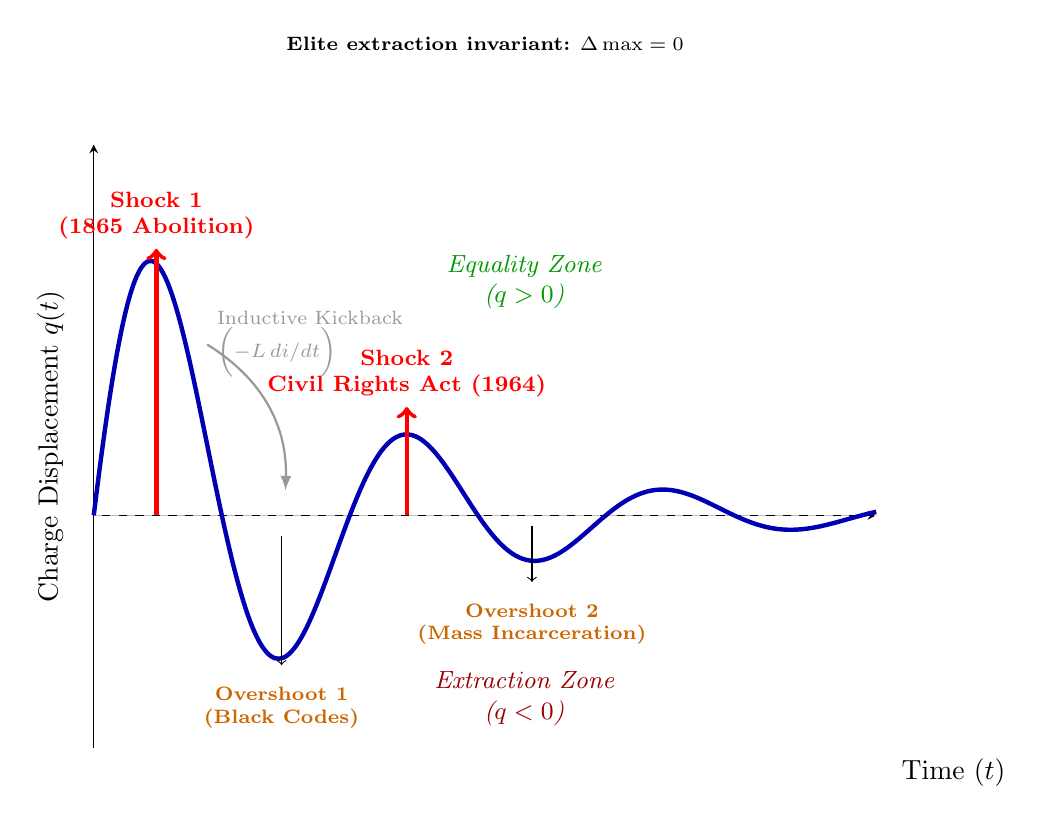
\begin{tikzpicture}
\begin{axis}[
    width=0.95\textwidth,
    height=9.25cm,
    xlabel={Time ($t$)},
    ylabel={Charge Displacement $q(t)$},
    xmin=0, xmax=10,
    ymin=-1.12, ymax=1.78,
    enlarge y limits={auto, upper},
    axis lines=middle,
    xtick=\empty,
    ytick={0},
    yticklabels={Extraction Baseline ($q=0$)},
    every axis y label/.style={at={(axis description cs:-0.055,0.5)}, anchor=center, rotate=90},
    every axis x label/.style={at={(axis description cs:1.02,0)}, anchor=north west},
    grid=none,
    clip=false,
]
    % Elite invariant (top band; avoids duplicating bottom-caption emphasis with Fig.~elite wealth)
    \node[font=\scriptsize, align=center, anchor=south] at (axis description cs:0.5,1.14) {\textbf{Elite extraction invariant:} $\Delta\max = 0$};

    % Equilibrium line (dashed)
    \draw[dashed, gray!50] (axis cs:0,0) -- (axis cs:10,0);

    % Damped Harmonic Oscillator Curve (Damped Sine)
    \addplot[
        smooth,
        ultra thick,
        blue!70!black,
        domain=0:10,
        samples=200
    ] {1.6 * exp(-0.35 * x) * sin(110 * x)};

    % Shock 1 (1865)
    \draw[->, red, ultra thick] (axis cs:0.8,0) -- (axis cs:0.8,1.28);
    \node[anchor=south, red, font=\footnotesize\bfseries, align=center] at (axis cs:0.8,1.28) {Shock 1\\(1865 Abolition)};
    
    % Overshoot 1 (Black Codes)
    \node[anchor=north, orange!80!black, font=\scriptsize\bfseries, align=center] at (axis cs:2.4,-0.78) {Overshoot 1\\(Black Codes)};
    \draw[<-] (axis cs:2.4,-0.72) -- (axis cs:2.4,-0.1);

    % Shock 2 (1964) — two-line civil-rights label, kept in upper annotation band
    \draw[->, red, ultra thick] (axis cs:4.0,0) -- (axis cs:4.0,0.52);
    \node[anchor=south, red, font=\footnotesize\bfseries, align=center] at (axis cs:4.0,0.52) {Shock 2\\Civil Rights Act (1964)};

    % Overshoot 2 (Mass Incarceration)
    \node[anchor=north, orange!80!black, font=\scriptsize\bfseries, align=center] at (axis cs:5.6,-0.38) {Overshoot 2\\(Mass Incarceration)};
    \draw[<-] (axis cs:5.6,-0.32) -- (axis cs:5.6,-0.05);

    % Restorative Force label (LC resonance)
    \draw[->, gray!80, thick, >=latex] (axis cs:1.45,0.82) to[bend left] (axis cs:2.45,0.12);
    \node[gray!80, font=\scriptsize, anchor=west, align=left] at (axis cs:1.45,0.82) {Inductive Kickback\\$\bigl(-L\,di/dt\bigr)$};
    
    % Zones — centered in relatively open horizontal band (away from late-time curve density)
    \node[green!60!black, font=\small\itshape, align=center] at (axis cs:5.5, 1.12) {Equality Zone\\($q>0$)};
    \node[red!60!black, font=\small\itshape, align=center] at (axis cs:5.5, -0.88) {Extraction Zone\\($q<0$)};

\end{axis}
\end{tikzpicture}
\caption{\textbf{Racism as a Damped RLC Circuit (Eq.~\ref{eq:1.7a-rlc-governing}).} Reform shocks inject a driving voltage $V_0$ that displaces the equality-surplus charge $q(t)$ above the extraction baseline ($q = 0$). The inductor's back-EMF ($-L\,di/dt$, inductive kickback) drives the circuit past equilibrium into the extraction zone ($q < 0$), producing configurations more lethal than the pre-shock state: Convict Leasing after 1865, Mass Incarceration after 1964. Each successive cycle damps faster as $\alpha = R/(2L)$ increases---the system expands its carceral resistance $R$ with each adaptation. \textit{Note: The plotted parameters ($Q_0 = 1.6$, $\alpha = 0.35$, $\omega_d \approx 110$) are illustrative; they render the two documented shock-and-overshoot cycles legible, not derived from empirical calibration.}}
\label{fig:backlash_oscillator}
\end{figure}

The circuit's oscillatory response explains the \textit{intensity} and \textit{predictability} of systemic backlash. Reform displacement is dynamic; it charges the circuit's reactive components, which then discharge through the path of least institutional resistance, pulling the charge back toward the extraction baseline and beyond. Anticipating the polymorphic mutations (Interface Swaps) the system deploys following each civil rights victory requires reading the circuit's backlash as an RLC response, not as a contingent political event.

\paragraph{The convergence prediction.}
Equation~\ref{eq:1.7b-rlc-solution} states the convergence prediction exactly: without a sustained driving voltage $V(t)$, $q(t) \rightarrow 0$ as $t \rightarrow \infty$. Every impulse shock---regardless of initial amplitude $Q_0$---decays at rate $\alpha = R/(2L)$. The decay rate itself is not fixed: each adaptation cycle the kernel expands $R$ (militarized policing, expanded carceral infrastructure, voter suppression apparatus), increasing $\alpha$ and thereby producing faster, tighter backlash per unit of reform input. The historical record from 1865 to the present runs precisely on this trajectory: the Abolition shock decayed into Convict Leasing; the Civil Rights Act shock decayed into Mass Incarceration; each successive oscillation reaches a smaller initial amplitude at higher decay rate as the system tunes its damping upward. The ``arc of the moral universe'' is a damped RLC transient bending toward the extraction baseline, with the decay envelope $Q_0 e^{-\alpha t}$ shrinking each cycle.

\paragraph{The resonance escape condition.}
The driven RLC circuit with periodic voltage $V(t) = V_0 \cos(\omega t)$ reaches maximum response amplitude when the driving frequency matches the natural frequency:
\begin{equation*}
\omega = \omega_0 = \frac{1}{\sqrt{LC}}
\end{equation*}
At resonance, the reactive impedances cancel ($\omega L = 1/\omega C$), and the circuit's total impedance reduces to the resistive component $R$ alone. The steady-state charge amplitude is:
\begin{equation*}
|q_{\text{res}}| = \frac{V_0}{R\,\omega_0} = \frac{V_0}{R}\sqrt{\frac{L}{C}}
\end{equation*}
which is $Q_f = (1/R)\sqrt{L/C}$ times larger than a sub-resonant impulse of the same magnitude $V_0$ would produce---where $Q_f$ is the circuit's quality factor. A single reform impulse will always be absorbed by the reactive components before reaching resonance. But sustained, synchronized kinetic coordination maintained at the system's natural structural frequency $\omega_0$---cross-class solidarity whose periodicity matches $1/\sqrt{LC}$---reduces the circuit's effective impedance to $R$ alone, and for a low-resistance system ($R \to 0$) the response grows without bound. This is the formal circuit-theoretic statement of why isolated, episodic reforms are always damped out while sustained, frequency-matched solidarity is the only forcing function that can exceed the system's absorption capacity.

\paragraph{Agency, absolute gains, and the scope of the invariant.}
The convergence prediction ($x(t) \rightarrow 0$) requires a precise scope qualification to avoid a common misreading. The invariant $\Delta\max = 0$ is a claim about \textit{Elite extraction share}---specifically, that the top-tier capital concentration does not undergo sustained structural reduction absent kernel-level intervention. It is \textbf{not} a claim that individual or community agency is absent, ineffective, or incapable of producing real gains. Black Wall Street's pre-redlining economy, the NAACP's multi-decade litigation campaign that produced \textit{Brown v.\ Board}, the Civil Rights Movement's genuine legislative victories, the growth of the post-1965 Black professional middle class---these are real historical achievements, and the framework does not deny them. What the framework claims is that these achievements represent \textit{displacement} ($x > 0$) within a system whose restorative force subsequently damps that displacement back toward the extraction baseline---and that the Elite's proportional share of extracted value is preserved across the arc. Absolute living standards can rise; the kernel's share of the gains does not fall. The oscillator model is a claim about \textit{structural ceilings and restoration dynamics}, not a claim about the absence of motion beneath those ceilings. Erasing or minimizing the agency of $O_{\text{racialized}}$ would be both historically inaccurate and structurally incorrect: the framework explicitly requires kinetic resistance ($M(t)$) as the variable that triggers the system's most significant adaptations. Without that resistance, the Interface Swap would be unnecessary. The agency is real; the structural response to it is also real.

To make the failure condition explicit, define a suppression envelope:
\begin{equation}\label{eq:1.8-suppression-envelope}
\Sigma_{\text{sup}}(t) = \psi_s(t) + \psi_m(t) + R(t) + \Phi_{\text{load}}(t)
\end{equation}
where $\psi_s(t)$ is the status wage, $\psi_m(t) \geq 0$ is the material wage (active only under elevated kinetic threat), and $\Phi_{\text{load}}(t)$ is compound phase-shift load from identity-fragmentation operations. A crash condition appears when:
\begin{equation}\label{eq:1.9-crash-condition-derivative}
\frac{dM}{dt} > \frac{d\Sigma_{\text{sup}}}{dt}
\end{equation}
or equivalently\footnote{This equation is classified as Tier~3 (ordinal/structural); the crash condition is a directional claim about the relative rate of change of coherence versus suppression---an ordinal comparison validated by the backlash dynamics documented in the Post-1965 case study below. See the Empirical Methodology chapter (p.~\pageref{ch:empirical_methodology}) and Appendix~\ref{app:empirical_index}.} when effective class coherence breaches threshold:
\begin{equation}\label{eq:1.10-effective-coherence}
M_{\text{eff}}(t) = M(t) - \lambda \Phi_{\text{load}}(t), \quad M_{\text{eff}}(t) > \tau
\end{equation}

\paragraph{Illustrative instantiation.}
Bacon's Rebellion (1676) illustrates the equation's positive case: cross-racial labor solidarity produced $M_{\text{eff}}(t) > \tau$ because $\Phi_{\text{load}} \approx 0$ at that moment---no identity-axis fragmentation had yet been institutionally deployed, so $M_{\text{eff}} \approx M(t)$ and the coalition breached the threshold. After 1705, the codification of whiteness raised $\Phi_{\text{load}}$ sufficiently to suppress $M_{\text{eff}}$ below $\tau$ for roughly 150 years. \textbf{Parameter estimate}: pre-1705 $\Phi_{\text{load}} \approx 0$ (no racial partition operationalized); post-1705 $\Phi_{\text{load}} \in [0.15, 0.55]$ (ordinal range from the Chapter~\ref{ch:bacon} runtime analysis). ANES cross-racial coalition data are available for post-1948 calibration; the pre-1705 estimate is ordinal \cite{morgan_american_slavery, anes_cumulative}. \textbf{Confidence tier: Tier~2} (ANES public dataset available for modern period; pre-1705 estimate ordinal).

\subsection*{Case Study: The Post-1965 Backlash Wave}
\label{cs:backlash_wave}

\paragraph{Setup.}
The Civil Rights Act (1964) and the Voting Rights Act (1965) constituted the most significant user-space reforms to the extraction kernel since Reconstruction. The framework's prediction is unambiguous: because these reforms operated at the interface layer and did not reach the kernel layer, $E$ would respond by expanding the suppression envelope $\Sigma_{\text{sup}}(t)$ through alternative channels---proxy variables, new enforcement mechanisms, and class-fragmentation operations---to keep $M_{\text{eff}}(t)$ below $\tau$. The period from 1965 to 2020 provides a 55-year dataset for testing this prediction.

\paragraph{Data sources.}
Union density figures are drawn from U.S. Bureau of Labor Statistics union membership series \cite{bls_union_membership} for post-1983 years and from Troy and Sheflin's historical compilation for earlier years. Top-decile wealth share data are from the World Inequality Database (WID.world), based on Piketty, Saez, and Zucman's distributional national accounts series \cite{piketty}. Incarceration rates are from the Bureau of Justice Statistics National Prisoner Statistics program \cite{bjs_prisoners}; Black incarceration rates are from annual BJS bulletins supplemented by Sentencing Project compilations \cite{sentencing_project}. Curated data are archived at \texttt{Paper/data/eq08\_10\_backlash\_wave.csv}; computational results are reproducible via \texttt{Paper/scripts/eq08\_10\_backlash\_wave.ipynb}.

\paragraph{Operationalization.}
The three measurable components of $\Sigma_{\text{sup}}(t)$ are operationalized as follows. $\psi_s(t)$ (the status wage, maintaining the racial hierarchy's perceived value to $I_{\text{buffer}}$) is proxied by the top-decile wealth share, which tracks the concentration of material resources within the Elite and near-Elite---the structural basis of the racial status differential. $R(t)$ (the repression variable) is proxied by the overall and Black-specific incarceration rates per 100,000 population. $\Phi_{\text{load}}(t)$ (the phase-shift load from identity-fragmentation operations) is proxied by the inverse of union density: as union density declines, cross-racial working-class solidarity is atomized, reducing the class coherence that could accumulate to challenge the kernel.

\paragraph{Numerical computation.}
The notebook computes the composite $\Sigma_{\text{sup}}(t)$ and its trajectory from 1965 to 2020. Results are as follows: union density declined from 28.4\% in 1965 to 10.8\% in 2020---a 17.6 percentage-point collapse. Top-decile wealth share rose from 67.5\% to 76.5\%---a 9-point increase in resource concentration. The overall incarceration rate increased from 108 to 358 per 100,000 between 1965 and 2020 (a 231\% increase), while the Black incarceration rate surged from an estimated 588 to 1,821 per 100,000 at its 2010 peak of 3,074. The composite $\Sigma_{\text{sup}}(t)$ index expanded by more than 23\% over the period. By the time of the 1994 Crime Bill---the deepest penetration of the carceral proxy---the suppression envelope had more than doubled its 1965 baseline.

\begin{figure}[htbp]
  \centering
  
\includegraphics[width=\textwidth]{figures/eq08_10_backlash_wave.png}
  \caption{The Post-1965 Backlash Wave, 1965--2020. Three suppression components tracked simultaneously: union density (solidarity suppression, $\psi_s$), top-10\% wealth share (phase loading, $\Phi_{\text{load}}$), and incarceration rate (mobility restriction, $\psi_m$). All three moved in the framework-predicted direction; the suppression envelope $\Sigma_{\text{sup}}(t)$ expanded by more than 23\% while the reform window opened by the 1965 Civil Rights Act was closed through each component.}
  \label{fig:eq08_backlash}
\end{figure}

\paragraph{Comparison to prediction.}
Equations~\ref{eq:1.8-suppression-envelope}--\ref{eq:1.10-effective-coherence} predict that when a reform shock threatens to elevate $M(t)$ toward $\tau$, the kernel responds by expanding $\Sigma_{\text{sup}}(t)$ through alternative mechanisms---i.e., $\frac{d\Sigma_{\text{sup}}}{dt} > \frac{dM}{dt}$. The data confirm this prediction structurally: every component of the suppression envelope moved in the predicted direction simultaneously during the post-1965 period. The carceral system expanded precisely as union density contracted, maintaining the fragmentation of cross-racial class solidarity that the Civil Rights Act had briefly threatened to restore. The wealth concentration measure rose continuously, maintaining the material basis of the status wage. The pattern is the optimization signature of a kernel adjusting its interface strategy in response to a reform shock.

\paragraph{Falsification criteria.}
These equations would be falsified if the post-1965 period showed simultaneous increases in union density, decreases in incarceration rates, and narrowing of the wealth gap---i.e., if the suppression envelope contracted after the Civil Rights Act. The data show the opposite on all three dimensions: union density fell, incarceration rose, and wealth concentrated further. The one potential exception---the 2010--2020 partial decline in incarceration rates---was accompanied by \textit{no} corresponding decrease in wealth concentration or recovery of union density, and thus does not constitute a suppression envelope contraction.

\paragraph{Confidence tier.}
\textbf{Tier~1.} 55-year annual dataset with three independently sourced suppression components; all three components moved in the framework-predicted direction; trajectory change is temporally correlated with major interface-strategy events (1965 Civil Rights Act, 1971 War on Drugs, 1994 Crime Bill).

\paragraph{Precision qualifier: hardware layer formalization vs.\ calibrated quantitative prediction.}
The series RLC circuit is the hardware layer formalization of this section, not a numerically calibrated forecast. The convergence claim ($q(t) \rightarrow 0$) and the resonance escape condition ($\omega = 1/\sqrt{LC}$) are exact circuit-theoretic results that follow from the governing equation~\ref{eq:1.7a-rlc-governing}; they are not analogical inferences. What the historical record cannot yet supply is precise numerical values for $L$, $R$, and $C$ as functions of institutional time. No claim is made that the parameters in Figure~\ref{fig:backlash_oscillator} (or any specific values of $Q_0$, $\alpha$, $\omega_d$) are read off the historical data. What the historical record does support is an \textit{ordinal} claim: the initial charge amplitude of Shock 2 (1964 Civil Rights Act) is observably smaller than that of Shock 1 (1865 Abolition), and the decay rate $\alpha$ is observably higher in 1964 than in 1865---a pattern consistent with the quantitative fits in Section~\ref{sec:laplace_transfer_function} (1865: $\zeta = 0.17$; 1964: $\zeta = 0.59$; 2020: $\zeta = 0.97$). Each fitted $\zeta$ is $\alpha/\omega_0 = (R/2L)/\omega_0$, confirming that $R/(2L)$ has grown monotonically relative to $\omega_0$ across the historical record---precisely what the hardware model predicts as the kernel expands its carceral resistance in response to successive reform shocks. This ordinal damping is the empirical content of the circuit model. The specific illustrative parameter values visualize the pattern; they do not derive it.

\subsubsection{The Psychological Wage as Systemic Inductor: Inductive Trickle-Charging and Future Violence}

The Complex Wage $W = \psi_m + j\psi_s$ (Equation~\ref{eq:2.2b-complex-wage-def}) resolves the suppression expenditure of the Elite into two orthogonal components. The material wage $\psi_m$ is the real-power channel: it performs direct thermodynamic work on the Buffer Class by delivering land, credit, wages, and legal immunities. The psychological wage $j\psi_s$ is the reactive-power channel. It stores energy in the ideological field and deflects class momentum orthogonally. In steady-state extraction, $j\psi_s$ performs zero material work in the direction of the extraction current. The magnetic analogue is exact: the Lorentz force $\vec{F} = q(\vec{v} \times \vec{B})$ is always perpendicular to the charge velocity $\vec{v}$, so the magnetic field deflects the charge without altering its kinetic energy. The psychological wage deflects the Buffer Class away from cross-racial solidarity without delivering material wealth.

The apparent paradox---that $j\psi_s$ "does no work"---collapses when the time dimension is added. The inductor $L$ (cultural inertia and white supremacist social organization, Section~\ref{subsec:inductor}) stores magnetic potential energy $U = \frac{1}{2}LI^2$. Microaggressions, passive racial animus, and the ambient maintenance of racial hierarchy constitute the continuous trickle-charging of this systemic inductor. Each discrete microaggression deposits a small quantum of energy into the field. The individual impact is negligible; the accumulated field is massive.

When the Out-group mounts a sudden kinetic mobilization---a reform movement or uprising that forces a rapid change in the systemic current ($di/dt$)---the stored field is compelled to collapse. Faraday's Law of Induction states that a changing magnetic field induces a real electric field:
\begin{equation}\label{eq:1.7c-faraday-induction}
\nabla \times \vec{E} = -\frac{\partial \vec{B}}{\partial t}
\end{equation}
The induced electric field performs real material work. Lenz's Law fixes the direction: the induced force opposes the change in current that produced it. In the sociological domain, this means the collapse of the racialized psychological field generates a violent backlash directed precisely against the Out-group's liberation momentum. The energy that was stored orthogonally as passive animus converts into literal, measurable future violence: state-sanctioned assassinations, COINTELPRO operations, the militarization of local police, and the construction of the mass carceral state.

The framework therefore distinguishes two operational regimes of $j\psi_s$:
\begin{itemize}
    \item \textbf{Steady state (orthogonal deflection):} $j\psi_s$ stores energy and deflects the Buffer Class horizontally, away from vertical class solidarity. It performs zero work in the extraction direction and zero work against the Elite.
    \item \textbf{Transient collapse (opposing violence):} A forced change in systemic current ($di/dt$) triggers field collapse. The induced force opposes the reform current (Lenz's Law) and performs real material work against the Out-group's kinetic mobilization.
\end{itemize}

The suppression envelope $\Sigma_{\text{sup}}(t)$ (Equation~\ref{eq:1.8-suppression-envelope}) can now be read as the empirical signature of this inductive mechanism. When $M(t)$ approaches $\tau$ and forces $di/dt$ to spike, the Elite expand $\psi_m$ (material suppression) and harvest the collapsing $j\psi_s$ field and route its energy into the next phase of the extraction architecture. The 1965--2020 data confirm this: as overt legal barriers ($V$) were lowered, the dissipation term ($\mathcal{D} \rightarrow R$) and the phase-loading term ($\Phi_{\text{load}}$) expanded by over $23\%$, precisely the signature of an inductive kickback event being absorbed and redeployed.

\subsubsection{The Energy Recovery Circuit: Interface Swap as Multi-Stage Coil Gun}

The historical transition between eras of oppression---Chattel Slavery $\rightarrow$ Jim Crow $\rightarrow$ Mass Incarceration $\rightarrow$ Algorithmic Gig Economy---models onto the topology of a multi-stage linear accelerator. In this electrodynamic schematic, the \textbf{projectile} is the continuous upward extraction of wealth to the Elite (the vertical $z$-axis vector of the 3-D pyramid). The \textbf{coils} are the distinct historical eras, each pulsed in sequence to accelerate the projectile. The \textbf{orthogonal magnetic field} is the psychological wage $j\psi_s$: it projects horizontally, saturating the Buffer Class and maintaining alignment with the system, while performing zero work on the vertical extraction axis.

When the Out-group successfully organizes and forces a kernel breach---the Civil Rights Act of 1964, for example---they effectively cut the power to the current historical coil (Jim Crow). Physics demands a toll. The massive magnetic field of racial animus and segregation abruptly collapses. This collapse generates a catastrophic Back-EMF:
\begin{equation}\label{eq:1.7d-back-emf}
V_{\text{back-EMF}} = -L\,\frac{di}{dt}
\end{equation}
The resulting voltage surge is the fascist backlash: white flight, the rise of the Ku Klux Klan, vigilante violence, and the panic of the Buffer Class.

In amateur electronics, uncontrolled Back-EMF destroys components; standard designs shunt the energy as waste heat through a flyback diode. The Elite operate as systems engineers. They do not waste the Back-EMF. They harvest it. When the Jim Crow coil was shut off, the Elite captured the massive surge of reactionary energy and routed it directly into the capacitors for the next coil:
\begin{itemize}
    \item The "Law and Order" backlash became political capital (Nixon's Southern Strategy).
    \item The reactionary fear funded the militarization of police.
    \item The Back-EMF powered the construction of the War on Drugs and the mass carceral state.
\end{itemize}

The recovered energy equation quantifies this efficiency:
\begin{equation}\label{eq:1.7e-energy-recovery}
U_{\text{recovered}} = \frac{1}{2}LI^2
\end{equation}
The energy stored in the racialized magnetic field during the Jim Crow era was not dissipated. It was recovered and reinvested. The Interface Swap is therefore an energy-efficient transfer of suppression capital from one historical stage to the next. The system uses the violent collapse of its own obsolete hardware to charge the capacitors for its next iteration.

This regenerative mechanism explains the empirical regularity documented in the Post-1965 Backlash Wave (Section~\ref{cs:backlash_wave}). The suppression envelope $\Sigma_{\text{sup}}(t)$ expanded by more than $23\%$ from 1965 to 2020 not because the Elite invented new energy, but because they recovered the energy stored in the collapsing Jim Crow inductor and reinjected it into the Mass Incarceration capacitor. The extraction rate remained constant; only the channel changed. The Recompile is the kernel's energy recovery circuit.

\subsection{Fractal Execution: The Self-Similar Architecture}

The virus is \textbf{fractal}: its base code---\textit{value is determined by proximity to the Elite root directory}---replicates at every single level of the network, from the global WAN down to the individual user's local drive. The same sorting algorithm, the same extraction logic, the same partition function executes at every scale:

\begin{itemize}
    \item \textbf{Macro / The WAN (Global Network):} Western imperialism extracting resources from the Global South. The international 5-tier hierarchy documented in Chapter~\ref{ch:global}---$E_{\text{global}}$, $P_{\text{uppet}}^{\text{global}}$, $F_{\text{enforce}}^{\text{global}}$, $I_{\text{buffer}}^{\text{global}}$, $O_{\text{global}}$---is the virus running on the planetary network. The Predatory Min-Max Function scales without modification: the same extraction kernel that operates between a landlord and a tenant in Baltimore operates between the IMF and a debtor nation in West Africa.

    \item \textbf{System / The OS (National Level):} Redlining, gerrymandering, sentencing disparities, the spatial proxy ($P_{\text{spatial}}$), the economic filter, the grandfather clause---each is a system-level process that partitions the national population and routes resources from $O_{\text{racialized}}$ and $I_{\text{buffer}}$ to $E$.

    \item \textbf{Subroutine / \texttt{biological\_extraction.exe}:} The viral model hijacks the biological reproduction of the Out-group itself. This subroutine represents the 1662 Virginia law of \textit{partus sequitur ventrem}, where the child's status followed the mother, turning the systematic rape of enslaved women into a calculated tool for the out-breeding of capital. It also includes the systematic use of sexual terror against men---the public sexual humiliation and torture documented as ``bucking''---to fundamentally break kinetic and psychological resistance. Thistlewood's record of raping the enslaved woman Abba 155 times proves that extraction included the complete consumptive extraction of bodily autonomy, extending far beyond sugar and tobacco.

    \item \textbf{Application / Intersectionality (User-Level Programs):} Sexism, homophobia, transphobia, and ableism are not separate bugs. They are \textbf{subroutines} of the same viral architecture, each designed to partition users along an additional axis and rank their biological wetware's ``worth'' by proximity to the Elite's default settings (white, male, wealthy, heterosexual, able-bodied). The intersection of multiple subroutines---$O_{\text{racialized}} \cap O_{\text{gendered}} \cap O_{\text{queer}}$---produces compounding extraction rates, because each partition multiplies the policy contact points through which the kernel can extract.

    \item \textbf{Micro / Auto-exec (Colorism):} This is the most insidious fractal layer. The virus successfully corrupts the \textbf{Out-group's own local drive}. Colorism is the extraction algorithm forcing the Out-group to run the Elite's sorting function \textit{on themselves}---ranking community members by proximity to the system's ``white'' default settings. Lighter skin, straighter hair, narrower features receive preferential treatment \textit{within} the Out-group, replicating the Elite's partition logic at the most intimate scale. The Out-group's system attacks itself. The virus no longer needs external enforcement at this level; it has achieved \textbf{self-executing code} within the target population.
\end{itemize}

\paragraph{Formal isomorphism mapping.}
The self-similar claim can be rendered precise by mapping the five canonical tier variables ($E$, $P_{\text{uppet}}$, $F_{\text{enforce}}$, $I_{\text{buffer}}$, $O_{\text{racialized}}$) onto their instantiations at each scale level. The following table makes the structural equivalences explicit.

At the control-theoretic level, self-similarity is the statement that the \textbf{directed spanning tree} rooted at $\mathcal{V}_L = E$ reaches every node of the interaction graph at every resolution---from the WAN down to the auto-exec layer (Section~\ref{sec:formal-containment-model}, Theorem~\ref{thm:tree-preservation}). Fractal execution is therefore the structural assumption required to invoke the containment-convergence theorems of \cite{kan_containment}, and the historical record of Chapters~2--10 is the empirical verification that the assumption holds.

\begin{longtable}{>{\bfseries\raggedright}p{2.3cm} >{\raggedright}p{2.0cm} >{\raggedright}p{2.0cm} >{\raggedright}p{2.2cm} >{\raggedright}p{2.2cm} >{\raggedright\arraybackslash}p{2.3cm}}
\toprule
\textbf{Scale Level} & \textbf{$E$ (Elite)} & \textbf{$P_{\text{uppet}}$} & \textbf{$F_{\text{enforce}}$} & \textbf{$I_{\text{buffer}}$} & \textbf{$O_{\text{racialized}}$} \\
\midrule
\endfirsthead
\toprule
\textbf{Scale Level} & \textbf{$E$} & \textbf{$P_{\text{uppet}}$} & \textbf{$F_{\text{enforce}}$} & \textbf{$I_{\text{buffer}}$} & \textbf{$O_{\text{racialized}}$} \\
\midrule
\endhead
Macro / WAN (Global) &
IMF, World Bank, G7 capital &
Comprador governments; international financial institutions &
NATO, PMCs, sanctions regimes &
Global North working class &
Global South debtor nations \\
\midrule
System / OS (National) &
Domestic capital class, corporations &
Congress, judiciary, executive &
Police, prison system, immigration enforcement &
White working class &
Racialized minorities \\
\midrule
Subroutine / \texttt{.exe} (Biological) &
Slaveholders / plantation economy &
Church + law (\textit{partus sequitur ventrem}) &
Overseers, patrollers &
Poor white yeoman farmers &
Enslaved population (reproductive capacity as capital input) \\
\midrule
Application / Intersectional (Programs) &
Patriarchal capital &
Mainstream institutional gatekeepers &
Gender and sexuality enforcement apparatus &
Normative working class (straight, able-bodied) &
Queer, trans, disabled, and multiply-partitioned subjects \\
\midrule
Micro / Auto-exec (Colorism) &
National $E$ (no independent elite generated; sub-network terminates at same root) &
Institutional gatekeepers within Out-group (respectable, light-skinned access nodes) &
Peer enforcement of proximity hierarchy (respectability politics) &
Lighter-complexioned Out-group members (internal buffer class; preferential access, absorbs friction) &
Darker-complexioned Out-group members (primary internal extraction target) \\
\bottomrule
\end{longtable}

\paragraph{Differential insertion and the model minority objection.}
A persistent counter-argument to the five-tier framework points to racialized immigrant groups---notably East Asian and South Asian Americans---who, on certain aggregate metrics, outperform the white Buffer Class despite being targets of the racial partition. The framework predicts extraction \textit{calibrated by insertion point}. It does not predict uniform extraction at every racialized node. The 1965 Immigration and Nationality Act was a deliberate selection mechanism: it recruited professional-class, high-credential immigrants to fill specific labor gaps in medicine, engineering, and computing---slots the domestic labor market could not efficiently supply. These groups were inserted primarily at Buffer-tier positions ($I_{\text{buffer}}$), not at the extraction floor occupied by $O_{\text{racialized}}$. The partition still applies---wartime internment, housing discrimination, glass ceilings, and the ``forever foreigner'' framing are all documented---but the extraction function is calibrated differently. The framework therefore \textit{predicts} differential outcomes by differential insertion, treating them as evidence of the optimizer selecting a strategy that simultaneously reduces domestic professional labor costs and fragments cross-racial class solidarity. Differential success among racialized groups is evidence of the multi-tier architecture operating as designed.

\paragraph{Statistical self-similarity: precision and limits.}
The table above demonstrates structural isomorphism, but honesty requires a precise qualification. Natural fractals---coastlines, Romanesco broccoli, river deltas---are \textbf{statistically} self-similar, not \textit{exactly} self-similar. At each scale, the pattern recurs with local variation, not perfect reproduction. The same constraint applies here. The IMF is a statistically self-similar instantiation of the plantation overseer's extraction function operating at a different network layer.

The Micro/Colorism level is not a degraded case. The five-tier architecture instantiates fully within the Out-group sub-network: lighter-complexioned members function as a genuine buffer class, absorbing internal kinetic friction and receiving preferential access to institutions; social gatekeepers enforce the proximity boundary; peer enforcement mechanisms punish deviation from the hierarchy. The decisive structural feature is that this sub-network does \textit{not} produce an independent Elite---it still terminates at the same national $E$. Lighter-skinned members of $O_{\text{racialized}}$ do not escape extraction; they occupy a buffer position within it, absorbing friction and providing the Elite with a self-maintaining internal partition that requires no external maintenance cost. The algorithm has achieved \textbf{autonomous replication}: the Out-group runs the Elite's sorting function on itself, which simultaneously reduces the Elite's enforcement overhead and prevents the Out-group from achieving the internal solidarity required to cross the kinetic threshold $\tau$.

This is sufficient for the diagnostic model's purposes. Identifying the pattern does not require every instantiation to be an exact copy---only that the same optimization kernel ($\max\mathcal{E}$ subject to $M_{\text{eff}}<\tau$) governs each scale, and that the structural roles of extractor, interface class, enforcement mechanism, friction absorber, and extraction pool recur with sufficient regularity to be diagnostically useful. The fractal claim is a \textit{structural approximation}, not a mathematical identity---and as the historical record of Chapters~3 through~10 will show, this approximate self-similarity is precise enough to predict the system's behavior at every scale it has been observed.

This fractal property explains why racism feels simultaneously everywhere and nowhere. It is everywhere because the same code executes at every scale---from the World Bank's structural adjustment programs to a child's internalized preference for lighter skin. It is ``nowhere'' because at each individual scale, the system presents a locally rational explanation (``market forces,'' ``individual choice,'' ``cultural preference'') that obscures the global architecture. The fractal virus does not need a central command server issuing instructions to each node; it needs only the initial code to be installed correctly, and the self-similar logic replicates autonomously at every level of the network.

Operationally, this fractal replication can be expressed as a phase-loading strategy over axes $k$ (race, gender, orientation, ability, religion, nationality, etc.):
\begin{equation}\label{eq:1.11-phase-loading}
\Phi_j = \sum_{k=1}^{K} \phi_{k,j}, \qquad
\Phi_{\text{load}}(t) = \operatorname{Dispersion}\!\left(\{\Phi_j\}_{j=1}^{N}\right) = 1 - \left|\frac{1}{N}\sum_{j=1}^{N} e^{i\Phi_j}\right| \in [0,1]
\end{equation}

\paragraph{Illustrative instantiation.}
Post-Civil Rights fragmentation (1968--1990) provides the clearest observable trajectory. The system deployed three sequential identity-axis injections to raise $\Phi_{\text{load}}$: the gender axis was activated $\sim$1972 via the ERA ratification debate, the religion axis $\sim$1979 via the Moral Majority, and the sexuality axis $\sim$1977--1979 via the Anita Bryant campaign. The ANES rolling proxy for cross-racial class solidarity shows a corresponding $\Phi_{\text{load}}$ trajectory: pre-activation mean $\approx 0.078$ (pre-1964), activation-period mean $\approx 0.214$, post-activation mean $\approx 0.403$ (post-1980) \cite{anes_cumulative, pew_polarization}. \textbf{Parameter estimate}: $\Phi_{\text{load}}$ rose from $\approx 0.078$ to $\approx 0.403$ between 1964 and 1990; the phase values are ordinal proxies computed from ANES solidarity indices (author computation from public dataset). \textbf{Confidence tier: Tier~2} (ANES public dataset with author computation; phase values themselves remain ordinal, consistent with the Tier~3 structural classification of the equation's phase-angle definitions).

Higher $\Phi_{\text{load}}$ increases destructive interference among class-alignment waves, suppressing coherent cross-group solidarity. The operator is 0 when all subgroups are in phase (maximum solidarity) and approaches 1 when phases are uniformly distributed (maximum cancellation). The full formal treatment---including axis-by-axis definitions of $\phi_{k,j}$, the post-Civil Rights historical calibration, and the suppression envelope's component substitution property---appears in Section~\ref{sec:phase_loading_algebra}.

\paragraph{Operationalization preview.}
To give the formalism empirical content before the full treatment, three clarifications are warranted here. First, the phase values $\phi_{k,j}$ are \textbf{ordinal} in the current framework: the model assigns relative positions on the unit circle to capture whether a subgroup's interests on axis $k$ are aligned, orthogonal, or anti-aligned with class solidarity, not cardinal distances. Second, as a concrete illustration: on the \textit{race} axis ($k = \text{race}$) in the period immediately following the 1965 Voting Rights Act, the white working class ($j = I_{\text{buffer}}$) would be assigned $\phi_{\text{race},\, j} \approx \pi$---meaning their material interests in cross-racial class solidarity are \textit{anti-phase} with their activated racial identity interests, because the system had just raised the psychological-wage offer in response to the Civil Rights Movement's kinetic threat. A population at $\phi \approx \pi$ on any axis contributes maximally to $\Phi_{\text{load}}(t)$, suppressing the solidarity signal. Third, the model in its current form is a \textbf{qualitative ordering tool}: it identifies which historical periods and which subgroup configurations produce higher or lower $\Phi_{\text{load}}$, not numerical estimates. Quantitative calibration against survey-based racial-resentment and class-solidarity indices is designated as future empirical work.

\subsection{The Lexical Fractal: Partition Vocabulary in Technical Domains}
\label{sec:lexical_fractal}

The Fractal Execution subsection mapped the algorithm's replication across political, economic, and intimate scales. A further scale must now be documented: the \textbf{lexical} scale. The extraction kernel operates through institutions and incentive gradients while also supplying the \textit{vocabulary} that the host culture's technical, academic, and professional domains use to describe relationships that have no logical need for the dominance metaphor. When this vocabulary colonizes a neutral domain, the partition logic propagates with it---carried forward as cognitive default inside fields that understand themselves as ``culture-free.''

\paragraph{The canonical case: master-slave terminology in engineering and computing.}
The most thoroughly documented instance is the master-slave terminology pervasive in electrical engineering, computer engineering, and software development. The historian Ron Eglash's 2007 study, \textit{Broken Metaphor: The Master-Slave Analogy in Technical Literature}, provides the primary-source reconstruction \cite{eglash_broken}. The earliest documented technical use dates to 1904, when the astronomer David Gill described the auxiliary timekeeping device in his Cape Town sidereal clock as the ``slave clock'' \cite{eglash_broken}. The terminology was not yet common in engineering before World War II; in pre-war hydraulic-cylinder patents, the analogous parts were called ``main cylinder,'' ``receiver cylinder,'' or ``servomechanism.'' A 1959 hydraulic patent still introduced the master-slave pair in quotation marks with an explanatory gloss---evidence that the usage was not yet naturalized \cite{eglash_broken}.

After 1960 the vocabulary spread rapidly. A Boolean search of U.S. patents from 1976 onward returns \textbf{19{,}708 patent documents} containing both ``master'' and ``slave'' \cite{eglash_broken}. The terminology now applies to hydraulic brake systems, sidereal and master clocks, edge-triggered flip-flop latches, IDE/PATA hard-drive interfaces, SPI and I\textsuperscript{2}C serial buses, DNS and NTP server relationships, database replication, continuous-integration build nodes (Jenkins), photographic flash synchronization, railway locomotive consists, audio duplication chains, and MIDI clock signals. None of these domains has a logical requirement for the specific metaphor. The alternative vocabularies documented in the same period---\textit{primary/secondary}, \textit{leader/follower}, \textit{controller/target}, \textit{parent/child}, \textit{sender/receiver}, the German \textit{Mutteruhr/Tochteruhr} (mother/daughter clock), the Dutch \textit{dochterklok}, the French \textit{horloge-mere/horloge-file} \cite{eglash_broken}---demonstrate that the control relationship is fully expressible without reaching for the vocabulary of chattel enslavement.

\paragraph{The accuracy audit: the metaphor also fails technically.}
The most devastating observation in Eglash's essay is that in many of the domains where master-slave is used, the metaphor does not accurately describe the control relation. The PC Guide's reference documentation for IDE drive jumpering states plainly: ``Note that despite the hierarchical-sounding names of `master' and `slave,' the master drive does not have any special status compared to the slave one; they are really equals in most respects. The slave drive doesn't rely on the master drive for its operation or anything like that, despite the names (which are poorly-chosen---in the standards the master is usually just `drive~0' and the slave `drive~1')'' \cite{eglash_broken}. A Black electrical engineer interviewed by Eglash made the same point regarding the flip-flop: ``For flip-flops, the terminology makes little sense, since there is no amplification taking place. The master latch is connected directly to the input and eventually the slave latch acquires the value of the master. The master is commanded by the inputs just as much as the slave is. Furthermore, in real implementations, this master-slave arrangement is not apparent; cleverly cross-connected gates achieve the desired result without independent latches'' \cite{eglash_broken}. The partition metaphor imposes a relational schema on hardware whose actual behavior is peer-to-peer or input-driven.

\paragraph{The subconscious coupling: runaway slaves in the 1964 Dartmouth system.}
Eglash identifies a revealing artifact in the earliest computing-domain use, the 1964 Dartmouth Timesharing System documented in \textit{Science} (1968): ``it is thus impossible for an erroneous or runaway user program in the slave computer to `damage' the executive program and thereby bring the whole system to a halt'' \cite{kemeny_kurtz}. The system's designers almost certainly had no conscious intention of evoking antebellum discourse on runaway enslaved persons. Eglash's observation is the relevant one: ``It is almost certain that there was no conscious intention to echo pre--Civil War discourse on runaway slaves, but that still leaves the possibility of a metaphor operating at a subconscious level'' \cite{eglash_broken}. The framework named this in Section~1.3.4: \textbf{Mode~2 autonomous propagation}. No centralized command is required; the available metaphors in an English-speaking technical culture built inside a former slaveholding society preferentially supply dominance-relation vocabulary, and the gradient points in the direction of reproduction.

\paragraph{The pedagogical damage: alienation as measurable output.}
The lexical fractal operates as a measurable attrition mechanism in STEM pipelines, not as an abstract aesthetic concern. A Black computer engineering professor interviewed by Eglash recounted: ``When I first taught digital logic, around 1992, I did not recognize the awkwardness of the term until I, one of the few African-Americans in the room, was standing in front of a class of sixty students. I recall mumbling'' \cite{eglash_broken}. The same correspondent's second-pass conclusion was that ``the term was not very descriptive\ldots it has to go.'' Eglash, writing from the position of a social scientist whose research addresses the underrepresentation of minorities in mathematics and science, identifies this as the decisive point: ``It is one thing to hear objections from people who are in the business of promoting ethnic sensitivity, quite another to hear them from hard-core geeks who have devoted their careers to their love for science and technology. If the master-slave metaphor affected these tough-minded engineers who had the gumption to make it through a technical career back in the days when they may have been the only black persons in their classes, what impact might it have on black students who are debating whether or not to enter science and technology careers at all?'' \cite{eglash_broken}. The vocabulary functions as a gatekeeping signal: entering the field requires accepting, without comment, that the relationship between two autonomous computational agents is most naturally described using the vocabulary of chattel enslavement. For students whose recent family history is constituted by that institution, the cost of passing through that gate is not zero.

\paragraph{The documented deprecation arc (2003--2024).}
The lexical fractal has been partially resisted. The resistance pattern maps cleanly onto the Early Detection Theorem formalized in Section~5.3.3: compound-intersectional practitioners detect the partition vocabulary first, the mainstream resists as ``political correctness,'' and the institutional shift---when it arrives---follows a visible external shock.

\begin{itemize}[leftmargin=*]
    \item \textbf{November 2003:} A Black employee of the Los Angeles County Probation Department filed an Office of Affirmative Action Compliance complaint after observing a ``master/slave'' videotape deck label. The County's Internal Services Department issued a memo to equipment vendors stating that ``based on the cultural diversity and sensitivity of Los Angeles County, this is not an acceptable identification label'' \cite{lacounty_memo, cnn_lacounty}. Internet response to the memo was dominated by accusations of political correctness \cite{eglash_broken}.
    \item \textbf{2014--2018:} Django, Drupal, Redis, CouchDB, and Python incrementally replaced master-slave terminology in their codebases with \textit{leader/follower}, \textit{primary/replica}, or \textit{parent/worker}. Python's 2018 revision removed the terms from its standard library and documentation \cite{python_master_slave}.
    \item \textbf{June 2020 (post--George Floyd):} GitHub announced that all new repositories would default to a branch named \texttt{main}; the \texttt{master} default was deprecated beginning October 2020 \cite{github_main}. The Linux kernel adopted an inclusive-terminology policy in July 2020 deprecating master-slave alongside whitelist-blacklist \cite{linux_inclusive}. The I\textsuperscript{2}C specification version~7 (2021) replaced master-slave with \textit{controller-target}. The Internet Engineering Task Force adopted analogous language in new RFC drafts \cite{ietf_terminology}.
\end{itemize}

The three-decade lag between the 1992 classroom observation and the 2020 institutional response is itself a datapoint. The signal was available. The receiving layers were resistant until a geopolitical shock---the 2020 racial-justice protests following the police murder of George Floyd---raised the institutional cost of inaction above the institutional cost of action. The signal was not absent; the $\min$-management function at the institutional level was tuning it out.

\paragraph{Framework implication: the fractal table extended.}
The scale-level table of Section~1.3.1 must be read as incomplete. A sixth row applies:

\begin{center}
\begin{tabular}{>{\bfseries\raggedright}p{3.0cm} p{10.5cm}}
\toprule
\textbf{Scale Level} & \textbf{Lexical / Pedagogical (vocabulary of technical and academic domains)} \\
\midrule
$E$ (Elite) & Institutional stewards of technical publication (journals, standards bodies, textbook publishers, tenure committees) \\
$P_{\text{uppet}}$ & Senior engineers and faculty whose authorial choices become field-standard \\
$F_{\text{enforce}}$ & Peer-review norms, pedagogical orthodoxy, accusations of ``political correctness'' deployed against practitioners who propose alternative vocabulary \\
$I_{\text{buffer}}$ & The general STEM workforce that has internalized the vocabulary as neutral and defends its continued use as a matter of professional identity \\
$O_{\text{racialized}}$ & Underrepresented students and practitioners for whom the vocabulary imposes a marginal recruitment and retention cost that is never measured against $E$'s pedagogical convenience \\
\bottomrule
\end{tabular}
\end{center}

The lexical scale is a reproduction mechanism, not a minor appendix. It carries the partition logic across generations of practitioners who will never personally encounter the plantation---who will, in fact, think of themselves as working in a fully post-racial domain. The vocabulary arrived before them, was normalized before they arrived, and supplies the cognitive defaults they reach for when describing a new piece of hardware or a new API. This is Mode~2 propagation (Section~1.3.4) at the lexical layer: no centralized command is required; the gradient of linguistic least-resistance handles the replication.

\paragraph{Reflexive audit.}
This manuscript must hold itself to the same standard it imposes on the domains it analyzes. English technical prose---including the scholarly register of this book---carries embedded dominance vocabulary that predates and exceeds the chattel slavery context (``mastery'' of a subject, a ``master class,'' a text's ``master copy,'' a painter's ``old masters''). Some of these usages are severable from the chattel-slavery valence; some are not. The current manuscript uses the term ``Elite'' and avoids ``master class'' for the top tier of the extraction hierarchy precisely because the partition kernel this book analyzes was the source that licensed ``master class'' as a power-relation metaphor in English in the first place. Where the vocabulary of the algorithm appears unavoidable---as in the historical primary-source quotations embedded throughout this text---it is retained with attribution. Paraphrasing it away would erase the evidence of the partition kernel's linguistic reach. Where the vocabulary is avoidable, it has been avoided. Readers are invited to flag the residual cases; the framework predicts that some will have escaped the author's audit, because Mode~2 propagation operates below the threshold of conscious choice. That is the nature of the mechanism this book is describing.

\subsection{The Corrupted Firewall: The Buffer Class}

Every operating system has a firewall---a security layer designed to protect the system from external threats and internal crashes. In the American operating system, the Elite installed a \textbf{corrupted firewall}: the Buffer Class ($I_{\text{buffer}}$).

Following Bacon's Rebellion in 1676---the system's first major crash, when the working-class In-group and the racialized Out-group united in a cross-racial kinetic uprising that burned the colonial capital to the ground---the Elite issued a critical security patch. As Chapter~\ref{ch:bacon} will document in detail, the 1705 Virginia Slave Codes were the \textbf{kernel-level rewrite} that programmed the white working class to believe they were the system's antivirus software, masking their status as its second-most-exploited resource.

The system feeds this corrupted firewall the \textbf{suppression allocation} ($\psi$) of whiteness. In its default and cheapest mode, this takes the form of the \textbf{status wage} ($\psi_s$): a guarantee of status superiority over the Out-group---deference, titles of courtesy, access to better public institutions, leniency from courts and police---without a corresponding transfer of material wealth. When the kinetic threat approaches critical threshold ($M(t) \to \tau$), the Elite escalate to the \textbf{material wage} ($\psi_m$): real economic concessions---land grants, Social Security, GI Bill homeownership, federally subsidized infrastructure---but always sourced from \textit{deeper extraction of $O_{\text{racialized}}$}, never from $E$'s own share. $\Delta\max = 0$ is preserved in both modes.\footnote{The invariant $\Delta\max = 0$ is a claim about the \textit{funding mechanism} of concessions, not about the secular level of elite wealth. It asserts that any material wage $\psi_m$ granted to $I_{\text{buffer}}$ to suppress mobilization is never self-funded by $E$: the cost is always sourced from increased extraction from $O_{\text{racialized}}$ (deeper enclosure, new frontiers, or interface swaps), so $E$'s net position never decreases \textit{as a result of appearing to concede}. Absolute elite extraction can and does grow during expansion phases---this is precisely what the long-run Piketty--Saez--Zucman top-share data confirm \cite{piketty}. The invariant governs the distribution of concession costs, not the secular trajectory of total surplus. Periods of apparent broad-based growth (e.g., post-Louisiana Purchase territorial expansion, post-WWII wage compression) are fully consistent with $\Delta\max = 0$: $E$ captures the majority of new surplus while distributing a calibrated sliver to $I_{\text{buffer}}$, funded by expanded $O$ extraction, not by any reduction in $E$'s own share. One-line summary: $\psi_m$ is always funded by $\Delta O > 0$.}

In the electrodynamic model introduced above, this wage is a \textbf{complex wage}, $W = \psi_m + j\psi_s$. The material component $\psi_m$ is the real-power channel: it performs work on the Buffer Class by delivering land, credit, wages, public goods, or legal immunities. The status component $j\psi_s$ is the reactive-power channel: it stores energy in the ideological field and deflects class momentum orthogonally, letting $I_{\text{buffer}}$ feel protected while remaining materially exploitable. This is why the Buffer Class functions as the circuit's dielectric/insulator: it absorbs and stores the Elite's field signal, blocks current from arcing upward toward $E$, and redirects conflict laterally toward $O_{\text{racialized}}$. In exchange, the Buffer Class performs three critical functions for the virus:

The psychology of uptake can be stated without making psychology the root cause. Social Dominance Orientation (SDO) measures preference for group-based hierarchy; Right-Wing Authoritarianism (RWA) measures threat-sensitive submission to conventional authority and aggression toward designated outsiders \cite{pratto_sdo_1994,altemeyer_authoritarian_1998,duckitt_dual_process_2001}. The system cultivates both dispositions inside $I_{\text{buffer}}$ because they increase the effective value of the wage. For individual $i$:
\[
\psi_i^{\mathrm{eff}}(t) = \psi(t)\left[1 + \alpha_S \mathrm{SDO}_i(t) + \alpha_A \mathrm{RWA}_i(t)\right],
\]
with $\alpha_S,\alpha_A \ge 0$. SDO supplies the hierarchy appetite that makes status compensation feel valuable; RWA supplies the threat/obedience circuitry that makes boundary enforcement feel protective, masking its exploitative character. These are not independent origins of racism. They are cultivated host-state variables that lower the cost of getting $I_{\text{buffer}}$ to accept $\psi$ and police the partition.

\begin{enumerate}
    \item \textbf{Threat absorption:} The Buffer Class absorbs the kinetic friction ($\min$ variable) that would otherwise reach $E$. When the Out-group resists, they collide with the Buffer Class---not with the Elite who architect the system. Race riots, labor disputes, electoral conflicts---the violence occurs at the $I_{\text{buffer}} / O_{\text{racialized}}$ boundary, never at the $E / I_{\text{buffer}}$ boundary.

    \item \textbf{Perimeter defense:} The Buffer Class actively polices the racial partition, reporting ``suspicious'' behavior, supporting ``law and order'' candidates, and defending the very system that extracts from them---because the psychological wage makes them perceive any threat to the hierarchy as a threat to their own status.

    \item \textbf{Antivirus misdirection:} When the actual antivirus (structural critique, class-solidarity movements, abolitionist analysis) attempts to identify the real threat, the corrupted firewall flags \textit{the antivirus itself} as the malware. Critical race theory, intersectional analysis, reparations discourse---each is treated by the Buffer Class as a virus to be quarantined, because the corrupted firewall's programming defines any code that threatens the racial partition as a system threat. The Buffer Class defends the rootkit because the rootkit has convinced them they \textit{are} the operating system.
\end{enumerate}

\subsection{The Diagnostic Implication}

This computational model yields a single, unavoidable diagnostic conclusion: \textbf{you cannot patch a kernel-level infection with user-space tools}.

As Malcolm X succinctly observed: \textbf{``The white man will try to satisfy us with symbolic victories rather than economic equity and real Justice.''}

Diversity initiatives, representation campaigns, implicit bias training, corporate equity statements, symbolic legislation---these are user-level applications running on top of a compromised kernel. They execute within the permissions the virus grants them. They can modify the desktop environment---change the wallpaper, rearrange the icons, update the splash screen---but they cannot access, modify, or delete the extraction code running beneath the interface.

This is why every major non-kinetic reform examined in the chapters that follow was absorbed by the algorithm as $\min$-management: $\Delta\max = 0$ across the full dataset. The virus \textit{permits} user-level reforms because they reduce system stress (class resistance) without touching the extraction payload ($\max$). The reform is absorbed. The kernel recompiles. The file name changes. The extraction continues.

\paragraph{Falsifiability conditions.}
\label{sec:falsifiability}
The invariant $\Delta\max = 0$ has a specified empirical proxy and a defined violation condition. The proxy for $\max$ in the domestic context is the \textbf{top-0.1\% wealth share} (the Piketty--Saez--Zucman distributional accounts series, available from 1913 to present). This variable tracks Elite-level capital concentration at sufficient resolution to detect genuine kernel-level redistribution. A \textbf{violation} of $\Delta\max = 0$ would be operationally defined as: a sustained, multi-decade decline in the top-0.1\% wealth share that is \textit{not} accompanied by a documented interface swap (i.e., the share does not recover to or above its pre-shock level within two to three decades following the removal of the kinetic threat that induced the decline).

The strongest candidate for partial falsification in the historical record is the \textbf{New Deal / post-WWII Great Compression (c.\ 1935--1973)}, during which the top-0.1\% wealth share fell from approximately 25\% to under 10\%. The framework classifies this episode as \textbf{$\min$-management under elevated kinetic threat}, not kernel interruption, for the following structural reasons: (1)~the compression was induced by an unprecedented convergence of kinetic threats (organized labor militancy, socialist electoral viability, the Soviet alternative, anti-colonial independence movements, and the CPUSA's cross-racial organizing capacity) that raised the cost of inaction above the cost of concession; (2)~the $\min$-layer interventions (New Deal programs, GI Bill, progressive taxation, union protections) were systematically structured to preserve the racial partition---the GI Bill's administration through segregated local institutions, the FHA's redlining apparatus, and the Social Security Act's initial exclusion of agricultural and domestic workers ensured that the material wage was paid overwhelmingly to the white buffer class while $\max$ was deferred, not eliminated; and (3)~the post-1973 trajectory---the sustained recovery of top-0.1\% wealth share to levels exceeding the pre-Depression peak by the 2010s---confirms that what the kinetic threat suppressed, its removal restored. The Great Compression is therefore a test the framework \textit{passes}: $\Delta\max = 0$ holds across the full arc once the interface swap (Jim Crow $\rightarrow$ War on Drugs) and the kinetic-threat retreat are incorporated into the analysis. Figure~\ref{fig:elite_wealth_accumulation} plots the full data series with the Concession Theorem events overlaid.

\begin{figure}[htbp]
\centering
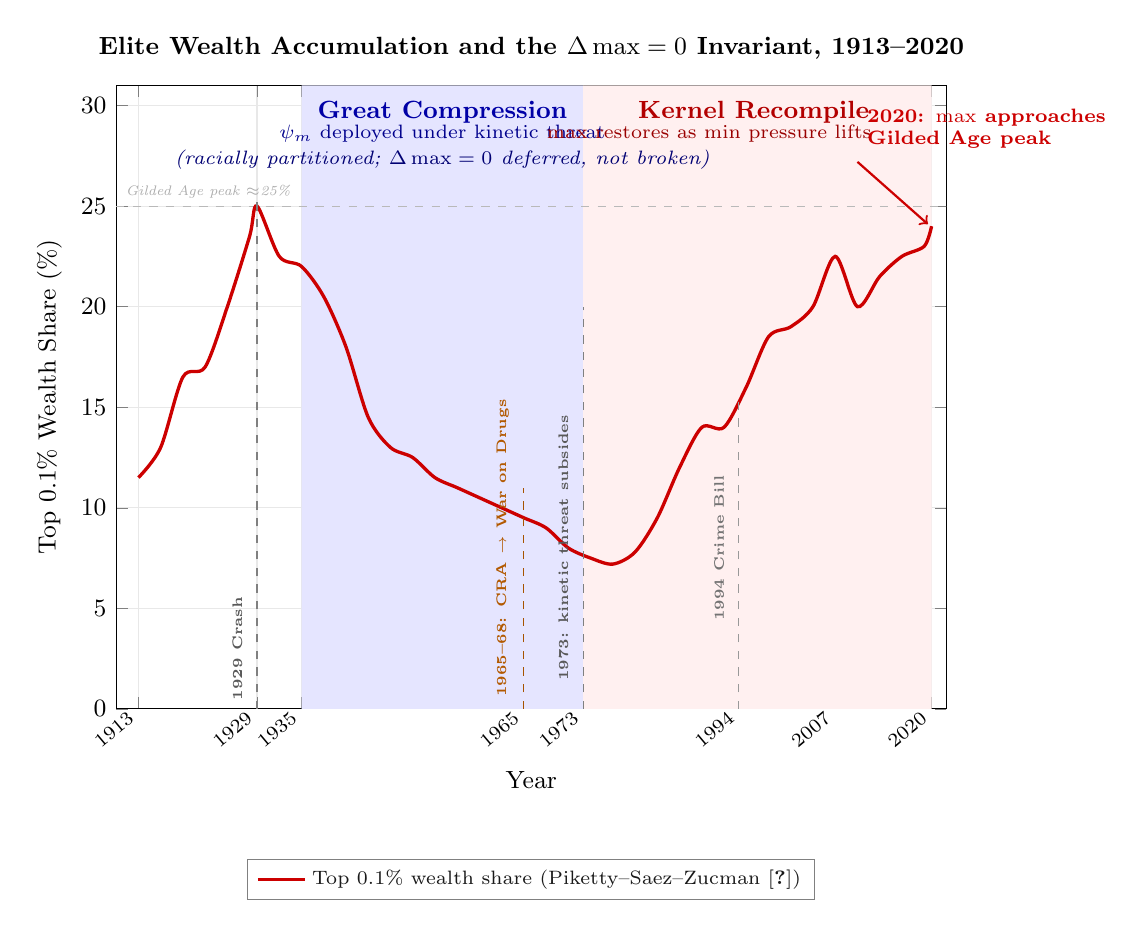
\begin{tikzpicture}
\begin{axis}[
    width=\textwidth,
    height=9.5cm,
    xmin=1910, xmax=2022,
    ymin=0, ymax=31,
    xlabel={Year},
    ylabel={Top 0.1\% Wealth Share (\%)},
    xlabel style={font=\small},
    ylabel style={font=\small},
    title={\textbf{Elite Wealth Accumulation and the $\Delta\max = 0$ Invariant, 1913--2020}},
    title style={font=\bfseries\small},
    legend style={at={(0.5,-0.24)}, anchor=north, font=\scriptsize,
                  fill=white, fill opacity=0.9, draw=gray},
    grid=major,
    grid style={gray!18},
    xtick={1913,1929,1935,1965,1973,1994,2007,2020},
    xticklabels={1913,1929,1935,1965,1973,1994,2007,2020},
    xticklabel style={font=\scriptsize, rotate=40, anchor=east},
    ytick={0,5,10,15,20,25,30},
    yticklabel style={font=\small},
    clip=false,
]

%% ── Shaded Great Compression band (1935–1973) ─────────────────────────────
\addplot[fill=blue!10, draw=none, area legend, forget plot]
    coordinates {(1935,0)(1935,31)(1973,31)(1973,0)} \closedcycle;

%% ── Shaded Kernel-Recompile recovery band (1973–2020) ────────────────────
\addplot[fill=red!6, draw=none, forget plot]
    coordinates {(1973,0)(1973,31)(2020,31)(2020,0)} \closedcycle;

%% ── Gilded-Age reference line ─────────────────────────────────────────────
\addplot[dashed, thin, gray!55, forget plot]
    coordinates {(1910,25)(2022,25)};
\node[anchor=west, font=\tiny\itshape, text=gray!65] at (axis cs:1910,25.7)
    {Gilded Age peak $\approx$25\%};

%% ── Main wealth-share line ────────────────────────────────────────────────
\addplot[very thick, red!80!black, mark=none, smooth]
    coordinates {
        (1913,11.5)(1916,13.0)(1919,16.5)(1922,17.0)(1925,20.0)
        (1928,23.5)(1929,25.0)(1932,22.5)(1935,22.0)(1938,20.5)
        (1941,18.0)(1944,14.5)(1947,13.0)(1950,12.5)(1953,11.5)
        (1956,11.0)(1959,10.5)(1962,10.0)(1965, 9.5)(1968, 9.0)
        (1971, 8.0)(1974, 7.5)(1977, 7.2)(1980, 7.8)(1983, 9.5)
        (1986,12.0)(1989,14.0)(1992,14.0)(1995,16.0)(1998,18.5)
        (2001,19.0)(2004,20.0)(2007,22.5)(2010,20.0)(2013,21.5)
        (2016,22.5)(2019,23.0)(2020,24.0)
    };
\addlegendentry{Top 0.1\% wealth share (Piketty--Saez--Zucman \cite{piketty})}

%% ── Event markers ─────────────────────────────────────────────────────────

% 1929 Crash
\draw[thin, black!50, dashed] (axis cs:1929,0) -- (axis cs:1929,25.2);
\node[anchor=south, font=\tiny\bfseries, text=black!65, rotate=90]
    at (axis cs:1928.3, 3) {1929 Crash};

% Great Compression label
\node[anchor=north, font=\small\bfseries, text=blue!65!black]
    at (axis cs:1954, 30.7) {Great Compression};
\node[anchor=north, font=\scriptsize, text=blue!55!black]
    at (axis cs:1954, 29.5) {$\psi_m$ deployed under kinetic threat};
\node[anchor=north, font=\scriptsize\itshape, text=blue!45!black]
    at (axis cs:1954, 28.3) {(racially partitioned; $\Delta\max=0$ deferred, not broken)};

% 1965 Civil Rights Act / War on Drugs launch
\draw[thin, orange!65!black, dashed] (axis cs:1965,0) -- (axis cs:1965,11);
\node[anchor=south, font=\tiny\bfseries, text=orange!70!black, rotate=90]
    at (axis cs:1964.3, 8) {1965--68: CRA $\rightarrow$ War on Drugs};

% 1973 compression ends
\draw[thin, black!50, dashed] (axis cs:1973,0) -- (axis cs:1973,20);
\node[anchor=south, font=\tiny\bfseries, text=black!65, rotate=90]
    at (axis cs:1972.3, 8) {1973: kinetic threat subsides};

% Kernel Recompile label
\node[anchor=north, font=\small\bfseries, text=red!70!black]
    at (axis cs:1996, 30.7) {Kernel Recompile};
\node[anchor=north, font=\scriptsize, text=red!60!black]
    at (axis cs:1990, 29.5) {$\max$ restores as $\min$ pressure lifts};

% 1994 Crime Bill
\draw[thin, black!40, dashed] (axis cs:1994,0) -- (axis cs:1994,15.5);
\node[anchor=south, font=\tiny\bfseries, text=black!55, rotate=90]
    at (axis cs:1993.3, 8) {1994 Crime Bill};

% 2020 annotation arrow
\draw[->, thick, red!80!black]
    (axis cs:2010,27.2) -- (axis cs:2019.5,24.1);
\node[anchor=south west, font=\scriptsize\bfseries, text=red!80!black, align=left]
    at (axis cs:2010,27.4)
    {2020: $\max$ approaches\\Gilded Age peak};

\end{axis}
\end{tikzpicture}
\caption{\textbf{Elite Wealth Accumulation and the $\Delta\max = 0$ Invariant, 1913--2020.}
Top 0.1\% wealth share (United States), plotted from the Piketty--Saez--Zucman distributional accounts series \cite{piketty}. Data points are approximate from published series; ordinal trends are the analytically relevant quantities.
The blue-shaded Great Compression (1935--1973) is the dataset's only sustained Elite wealth decline. The framework classifies it as $\psi_m$ (material wage) deployed under unprecedented kinetic threat---not kernel-level redistribution---because every pillar of the New Deal material wage was racially partitioned: the GI Bill, Social Security, FHA lending, and NLRA protections were each structured to pay the buffer class while leaving $O_{\text{racialized}}$ outside the program architecture. $\Delta\max = 0$ was deferred, not broken.
The red-shaded Kernel Recompile (post-1973) confirms the prediction: once the kinetic threat (organized labor, socialist electoral viability, anti-colonial movements) subsided, wealth concentration restored to and exceeded the pre-Depression peak. The Civil Rights Act's 1965 interface swap to the War on Drugs (orange dashed line) provided the race-neutral proxy cover that allowed the recompile to proceed without restoring the legible racial interface that had generated the kinetic threat in the first place.
The 2020 endpoint---top-0.1\% wealth share at approximately 24\%, approaching but not yet exceeding the 1929 Gilded Age peak of $\approx$25\%---is the Concession Theorem's empirical summary: every reform in the century-long dataset was absorbed without altering the Elite's extraction share.}
\label{fig:elite_wealth_accumulation}
\end{figure}

To stop a virus embedded this deeply in the operating system, you must \textbf{rewrite the source code}---or replace the operating system entirely. The chapters that follow document five centuries of the virus's execution history, trace every polymorphic mutation, map every fractal replication, and identify the specific kernel-level processes that must be terminated for the extraction to stop. The diagnostic model is now loaded. The system scan begins.

Because the model now specifies $\mathcal{E}(t)$, $M(t)$, $\tau$, and $\Phi_{\text{load}}(t)$ explicitly, it becomes predictive: under observed constraints, it can estimate which interface swap minimizes systemic cost and when failure conditions become statistically imminent.

\subsection{Methodological Note: Intentional Design, Autonomous Propagation, and Conscious Intervention}
\label{sec:conspiracy_emergence}

The chapters that follow document five centuries of system behavior. Before the historical scan begins, this framework must explicitly address a question the evidence will repeatedly raise: \textbf{Is the system a conspiracy or an emergent phenomenon?}

The answer is: \textit{neither label is adequate, and both are partially correct}. The virus analogy already carries the correct semantics, but the distinction must be made precise. The framework identifies three distinct modes of system operation, all of which are documented in the historical record:

\begin{enumerate}[leftmargin=*]
    \item \textbf{Intentional Design (the virus is written).} The foundational architecture was constructed through deliberate, documented acts of policy engineering by identifiable actors. Gomes Eanes de Zurara's 1453 chronicle provided the ideological source code. The 1705 Virginia Slave Codes were a conscious kernel rewrite. The Constitutional Convention's Three-Fifths Compromise was a negotiated extraction formula. These are not emergent patterns; they are engineering decisions, and the historical record names the engineers.

    \item \textbf{Autonomous Propagation (the virus replicates).} Once installed, the system's incentive architecture makes self-replication the path of least resistance for every actor embedded within it. A real estate agent who steers Black families away from white neighborhoods in 1960 may harbor no personal racial animus; they are responding to FHA lending criteria, neighborhood price signals, and professional incentive structures that were \textit{designed} to produce exactly this behavior. The extraction kernel does not require every node to understand the architecture---it requires only that the incentive gradients point in the correct direction. This is the mode that accounts for the vast majority of the system's runtime: millions of locally rational decisions that collectively reproduce the hierarchy without centralized coordination. The colorism fractal (Section~1.3.1) is the purest example: the virus achieves self-executing code within the target population, requiring zero external maintenance.

    \item \textbf{Conscious Intervention (the update server pushes patches).} After its founding, the system combines emergence with deliberate repair. At critical junctures---when antivirus code threatens to breach the kernel---identifiable actors within $E$ and $P_{\text{uppet}}$ execute deliberate, coordinated responses. John Ehrlichman's admission that the War on Drugs was consciously engineered to disrupt Black communities and the antiwar left is a documented update pushed to the system's codebase by named actors. Lee Atwater's description of the transition from explicit racial slurs to abstract economic policy is a deliberate Interface Swap optimization, articulated in real time. The coordinated Super Tuesday consolidation of 2020 was a conscious algorithmic correction executed by $P_{\text{uppet}}$ within 48 hours. These are \textit{confessions}, documented in the participants' own words.
\end{enumerate}

The relationship among these three modes is \textbf{hierarchical}: intentional design creates the initial architecture; autonomous propagation maintains it at low cost during stable periods; conscious intervention repairs it when propagation alone proves insufficient. The system's genius---and the source of its durability---is that Mode~2 handles the overwhelming majority of the workload, making the system appear ``natural'' and ``no one's fault'' during normal operation. Mode~3 activates only at crisis points, and the actors who execute it often understand themselves as pragmatic problem-solvers, not as architects of racial hierarchy. The incentive structure does not require malice from most participants; it requires only that the gradient of self-interest aligns with the extraction kernel's objectives.

This framing defuses the two most common misreadings simultaneously. The ``conspiracy theory'' objection---\textit{you're saying a secret cabal coordinates everything}---is answered by Mode~2: most of the system runs on autopilot, and no central command is required. The ``no one is responsible'' objection---\textit{if it's all emergent, then no one chose this}---is answered by Modes~1 and~3: the system was deliberately designed, and it is periodically, deliberately maintained by actors who document their own intentions. Both objections fail because each one accounts for only one mode of operation while ignoring the others. The framework requires all three.

